%%%%%%%%%%%%%%%%%%%%%%%%%%%%%%%%%%%%%%%%%
% Beamer Presentation
% LaTeX Template
% Version 1.0 (10/11/12)
%
% This template has been downloaded from:
% http://www.LaTeXTemplates.com
%
% License:
% CC BY-NC-SA 3.0 (http://creativecommons.org/licenses/by-nc-sa/3.0/)
%
%%%%%%%%%%%%%%%%%%%%%%%%%%%%%%%%%%%%%%%%%

%----------------------------------------------------------------------------------------
%	PACKAGES AND THEMES
%----------------------------------------------------------------------------------------

\documentclass{beamer}

\mode<presentation> {

% The Beamer class comes with a number of default slide themes
% which change the colors and layouts of slides. Below this is a list
% of all the themes, uncomment each in turn to see what they look like.

%\usetheme{default}
%\usetheme{AnnArbor}
%\usetheme{Antibes}
%\usetheme{Bergen}
%\usetheme{Berkeley}
%\usetheme{Berlin}
%\usetheme{Boadilla}
%\usetheme{CambridgeUS}
%\usetheme{Copenhagen}
%\usetheme{Darmstadt}
%\usetheme{Dresden}
%\usetheme{Frankfurt}
%\usetheme{Goettingen}
%\usetheme{Hannover}
%\usetheme{Ilmenau}
%\usetheme{JuanLesPins}
%\usetheme{Luebeck}
\usetheme{Madrid}
%\usetheme{Malmoe}
%\usetheme{Marburg}
%\usetheme{Montpellier}
%\usetheme{PaloAlto}
%\usetheme{Pittsburgh}
%\usetheme{Rochester}
%\usetheme{Singapore}
%\usetheme{Szeged}
%\usetheme{Warsaw}

% As well as themes, the Beamer class has a number of color themes
% for any slide theme. Uncomment each of these in turn to see how it
% changes the colors of your current slide theme.

%\usecolortheme{albatross}
%\usecolortheme{beaver}
%\usecolortheme{beetle}
%\usecolortheme{crane}
%\usecolortheme{dolphin}
%\usecolortheme{dove}
%\usecolortheme{fly}
%\usecolortheme{lily}
%\usecolortheme{orchid}
%\usecolortheme{rose}
%\usecolortheme{seagull}
%\usecolortheme{seahorse}
%\usecolortheme{whale}
%\usecolortheme{wolverine}

%\setbeamertemplate{footline} % To remove the footer line in all slides uncomment this line
%\setbeamertemplate{footline}[page number] % To replace the footer line in all slides with a simple slide count uncomment this line

%\setbeamertemplate{navigation symbols}{} % To remove the navigation symbols from the bottom of all slides uncomment this line
}

\usepackage{graphicx} % Allows including images
\usepackage{booktabs} % Allows the use of \toprule, \midrule and \bottomrule in tables
\usepackage[utf8]{inputenc}
\usepackage{xcolor}

%----------------------------------------------------------------------------------------
%	TITLE PAGE
%----------------------------------------------------------------------------------------

\title[Visualização de Software - Mezuro]{Análise exploratória do projeto
Mezuro: uma proposta de evoluç\~ao e aplicaç\~ao de técnicas de Visualizaç\~ao
de Software}
% The short title appears at the bottom of every slide, the full title is only
% on the title page

\author{Álvaro Fernando M. de Souza} % Your name
\institute[UnB-FGA] % Your institution as it will appear on the bottom of every slide, may be shorthand to save space
{
Universidade de Brasília - Faculdade Gama \\ % Your institution for the title page
\medskip
\textit{alvarofernandoms@gmail.com} % Your email address
}
\date{Janeiro, 2016} % Date, can be changed to a custom date

\begin{document}

\begin{frame}
\titlepage % Print the title page as the first slide
\end{frame}

\begin{frame}
\frametitle{Agenda} % Table of contents slide, comment this block out to remove it
\tableofcontents % Throughout your presentation, if you choose to use \section{} and \subsection{} commands, these will automatically be printed on this slide as an overview of your presentation
\end{frame}

%----------------------------------------------------------------------------------------
%	PRESENTATION SLIDES
%----------------------------------------------------------------------------------------

%------------------------------------------------
\section{Introdução} % Sections can be created in order to organize your presentation into discrete blocks, all sections and subsections are automatically printed in the table of contents as an overview of the talk
%------------------------------------------------

\subsection{Questionamento}

\begin{frame}
\frametitle{Introdução}
Questionamento inicial: \\
\begin{itemize}
\item Qual método do seu sistema é o mais chamado?
\item Como aferir a qualidade de um código?
\item O quão complexo é entender o seu sistema?
\end{itemize}
A visualização de software pode auxiliar e ou facilitar o entendimento destes aspectos, e pode reduzir essa complexidade.
\end{frame}

%------------------------------------------------
\section{Visualização de Software} % Sections can be created in order to organize your presentation into discrete blocks, all sections and subsections are automatically printed in the table of contents as an overview of the talk
%------------------------------------------------

\begin{frame}
\frametitle{Visualização de Software}
\center
\textit{“Imagination or visualization, and in particular the use \\
of diagrams, has a crucial part to play in scientific research.”} \\
\centerline{René Descartes, 1637.}
\end{frame}

%------------------------------------------------

\begin{frame}
\frametitle{Visualização de Software}

\begin{itemize}
\item Computação Gráfica
\end{itemize}

O estudo da visualização de um dado pode ser dividido em dois ramos:
\begin{itemize}
\item Visualização Científica
\item Visualização de Informação:
\begin{itemize}
\item Grandes conjuntos de dados
\item Envolve algo mais complexo
\end{itemize}
\end{itemize}
\end{frame}

%------------------------------------------------

\begin{frame}
\frametitle{Visualização de Software}
\center Quantos números 3 existem abaixo?

\center
1281768756138976546984506985604982 \\
826762 9809858458224509856458945098450980 \\
943585 9091030209905959595772564675050678 \\
904567 8845789809821677654876364908560912 \\
949686 6138976546984506985604982 \\
826762 98098584582245098 \\

\end{frame}

%------------------------------------------------

\begin{frame}
\frametitle{Visualização de Software}
\center Quantos números 3 existem abaixo?

\center
12817687561\textcolor{red}{3}8976546984506985604982 \\
826762 9809858458224509856458945098450980 \\
94\textcolor{red}{3}585 90910\textcolor{red}{3}0209905959595772564675050678 \\
904567 8845789809821677654876\textcolor{red}{3}64908560912 \\
949686 61\textcolor{red}{3}8976546984506985604982 \\
826762 98098584582245098 \\

\end{frame}

%------------------------------------------------

\begin{frame}
\frametitle{Visualização de Software}
\begin{itemize}
\item Visualização de Informação \textgreater Visualização de Software
\item Auxiliar a compreensão de sistemas complexos
\item Aumentar a produtividade
\end{itemize}

\end{frame}

%------------------------------------------------
\section{Categorias da Visualização de Software} % Sections can be created in order to organize your presentation into discrete blocks, all sections and subsections are automatically printed in the table of contents as an overview of the talk
%------------------------------------------------

\begin{frame}
\frametitle{Categorias da VS}
\begin{itemize}
\item Estrutura
\item Comportamento
\item Evolução
\end{itemize}

\end{frame}

%------------------------------------------------

\begin{frame}
\frametitle{Categorias da VS - Estrutura}

\center
Relacionada ao que é estático em um software, sem necessidade de executá-lo. Por exemplo: o código-fonte, as estruturas de dados do programa, o grafo de chamadas estático e a organização do sistema em módulos.

\end{frame}

%------------------------------------------------

\begin{frame}
\frametitle{Categorias da VS - Estrutura}

\begin{figure}[!htb]
  \centering
    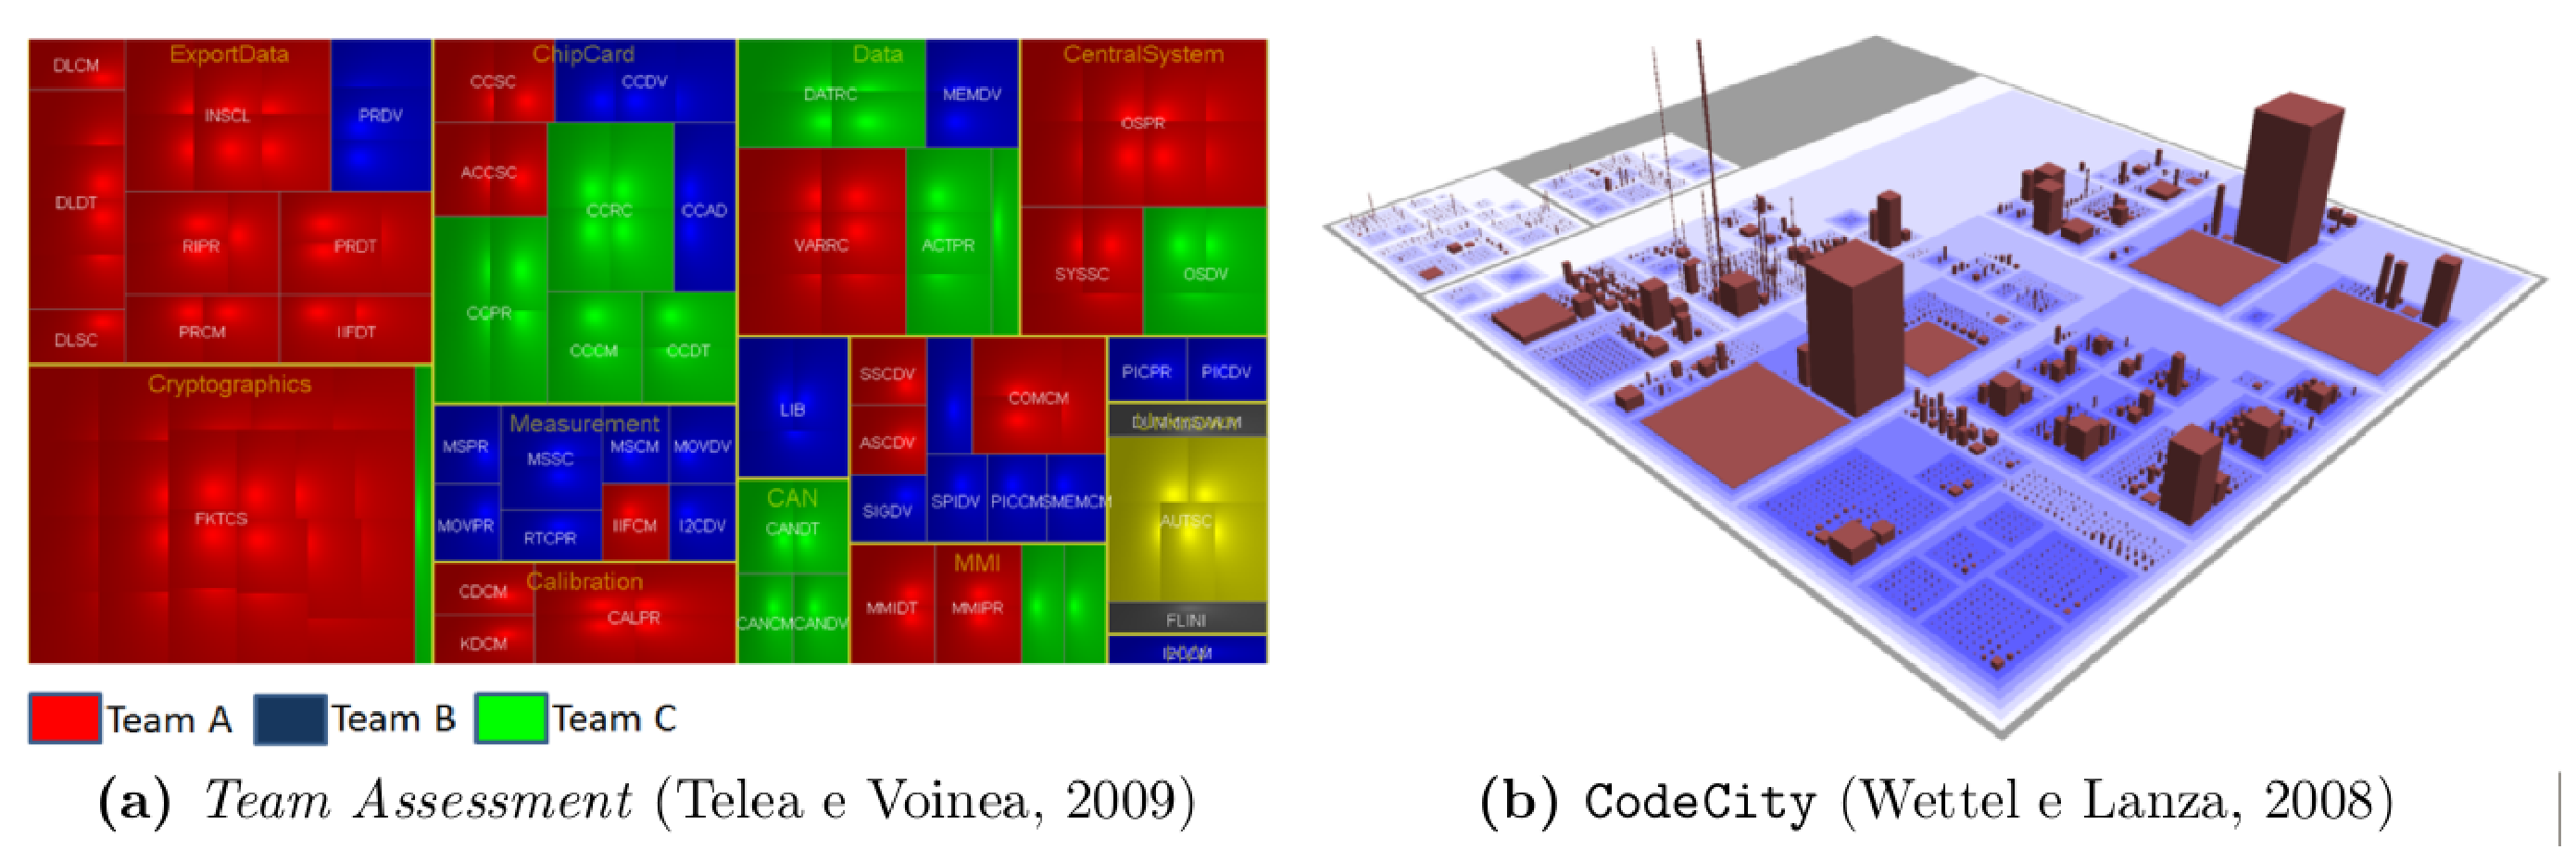
\includegraphics[keepaspectratio=true,scale=0.26]
    {../figuras/codeTeam_codeCity.eps}
  \caption{Exemplo Categoria Estrutura \cite{messias2012}}
  \label{fig:parallel}
\end{figure}


\end{frame}

%------------------------------------------------

\begin{frame}
\frametitle{Categorias da VS - Comportamento}

\center
O software é executado. Análise do que acontece, em tempo de execução, dada determinada entrada. Técnica: sequência de estado. Combinar dados e código para analisar interação com a memória. Dependendo do paradigma de programação, pode haver uma relação entre os métodos ou funções e a comunicação entre os objetos.


\end{frame}

%------------------------------------------------

\begin{frame}
\frametitle{Categorias da VS - Comportamento}

\begin{figure}[!htb]
  \centering
    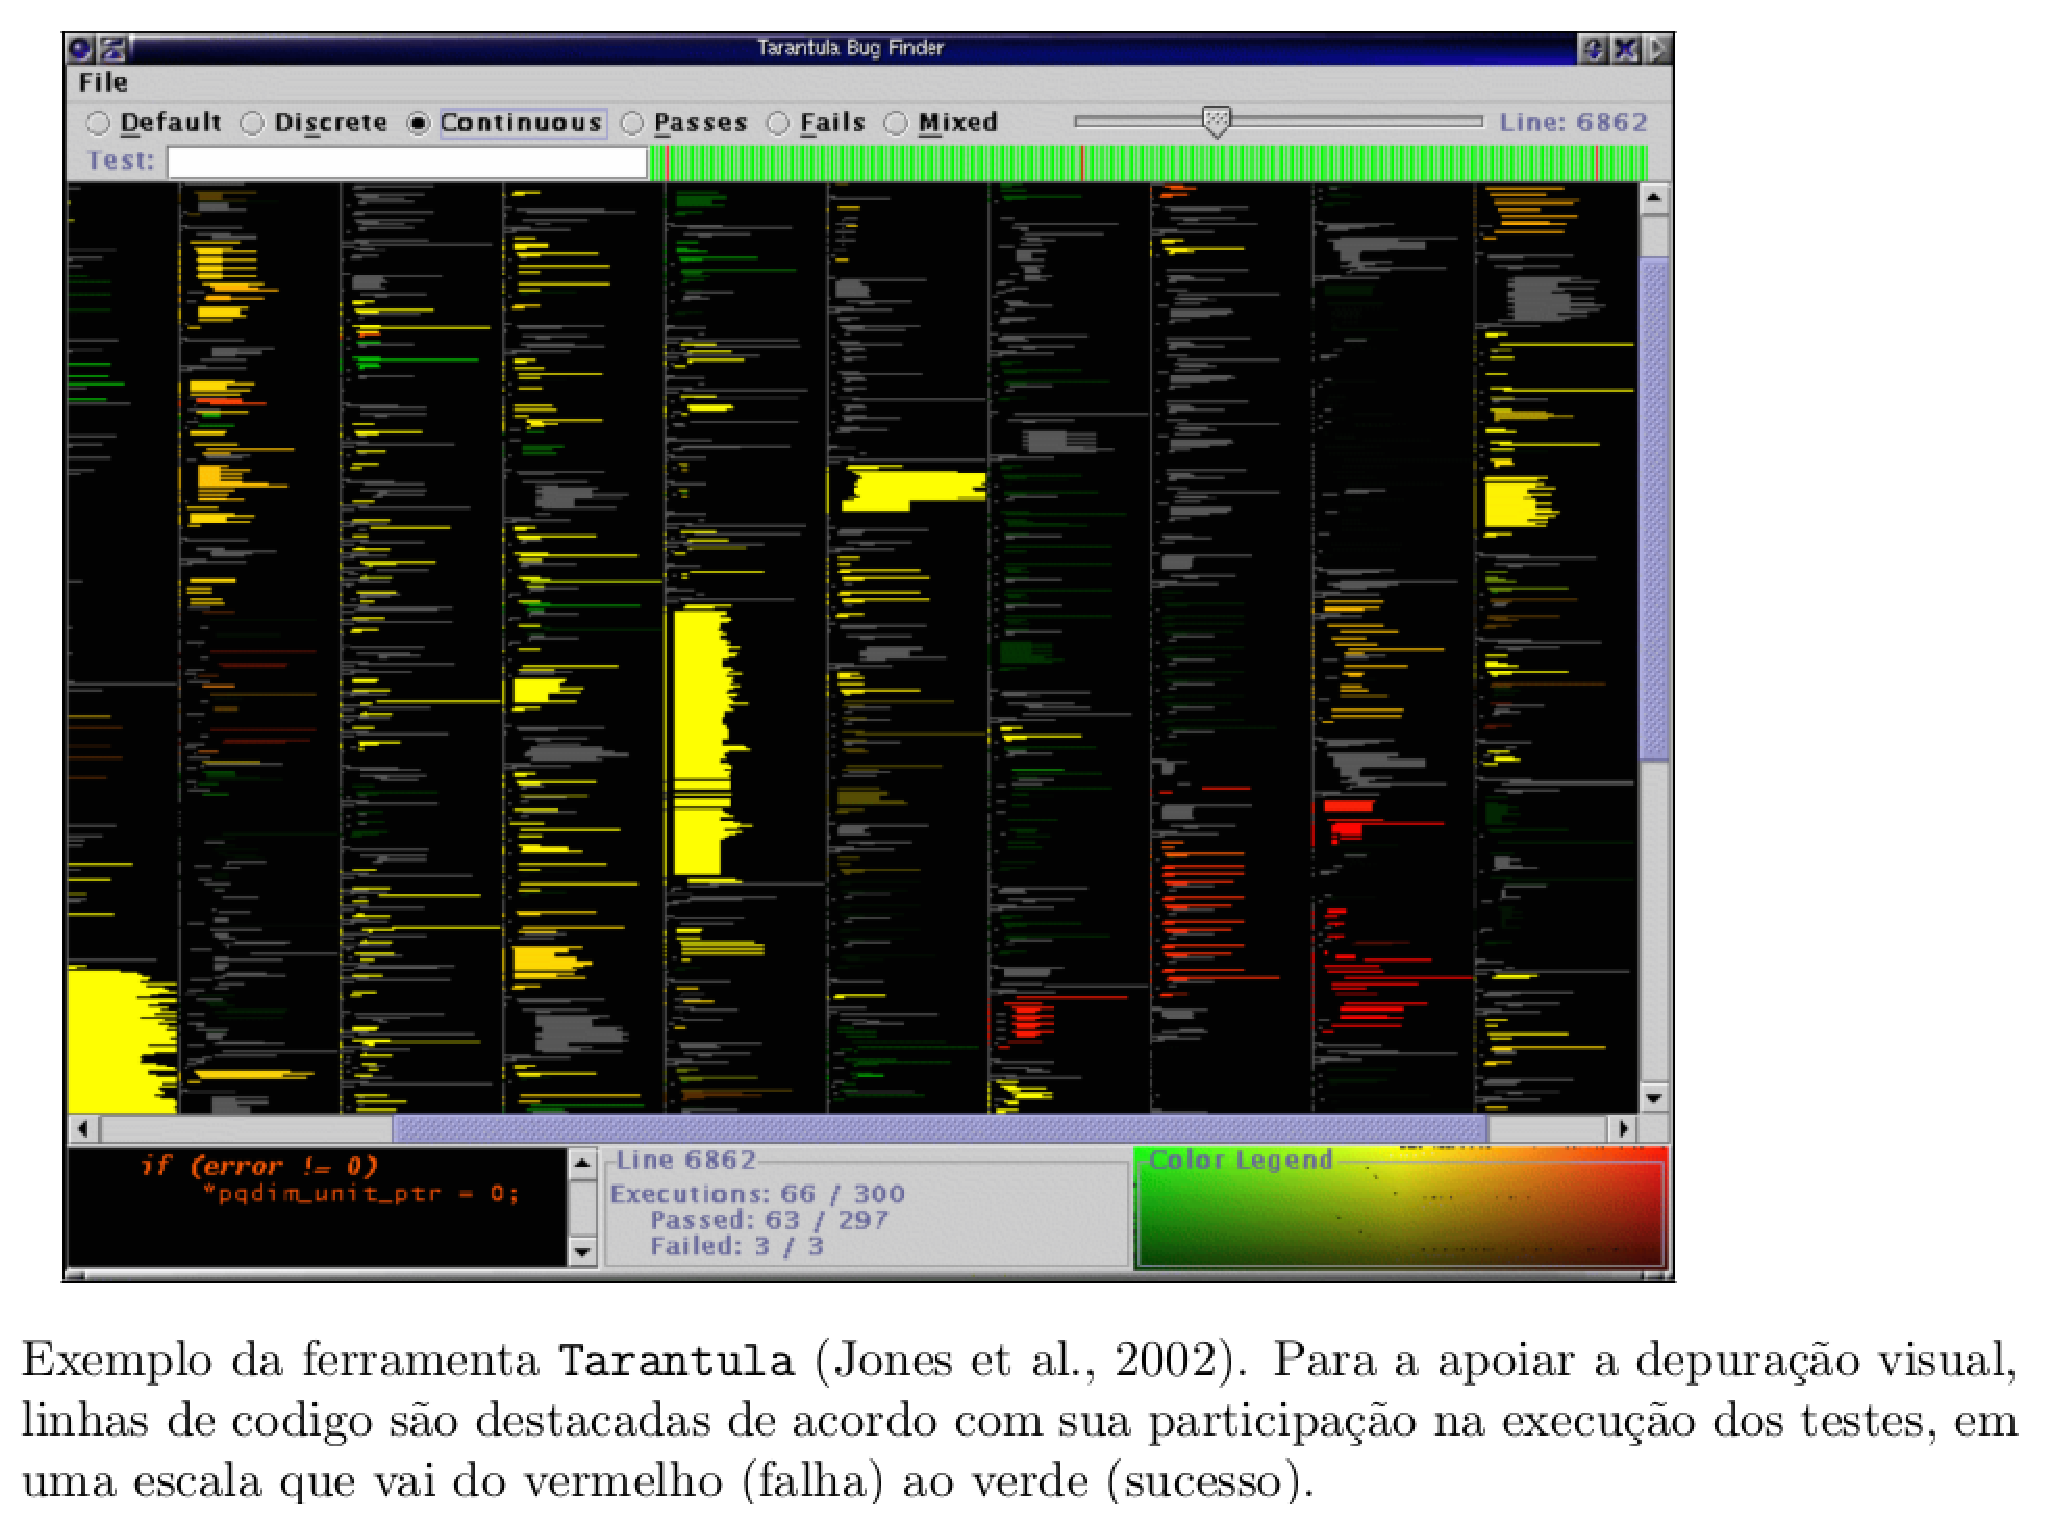
\includegraphics[keepaspectratio=true,scale=0.26]
    {../figuras/exemplo_tarantula.eps}
  \caption{Exemplo Categoria Comportamento \cite{messias2012}}
  \label{fig:parallel}
\end{figure}


\end{frame}

%------------------------------------------------

\begin{frame}
\frametitle{Categorias da VS - Evolução}

\center
Categoria aplicada para compreensão das modificações ao longo do tempo. A manutenção e evolução de um sistema pode chegar a 80\% do custo total de desenvolvimento. Dado este que fortalece as visualizações desta categoria.


\end{frame}

%------------------------------------------------

\begin{frame}
\frametitle{Categorias da VS - Evolução}

\begin{figure}[!htb]
  \centering
    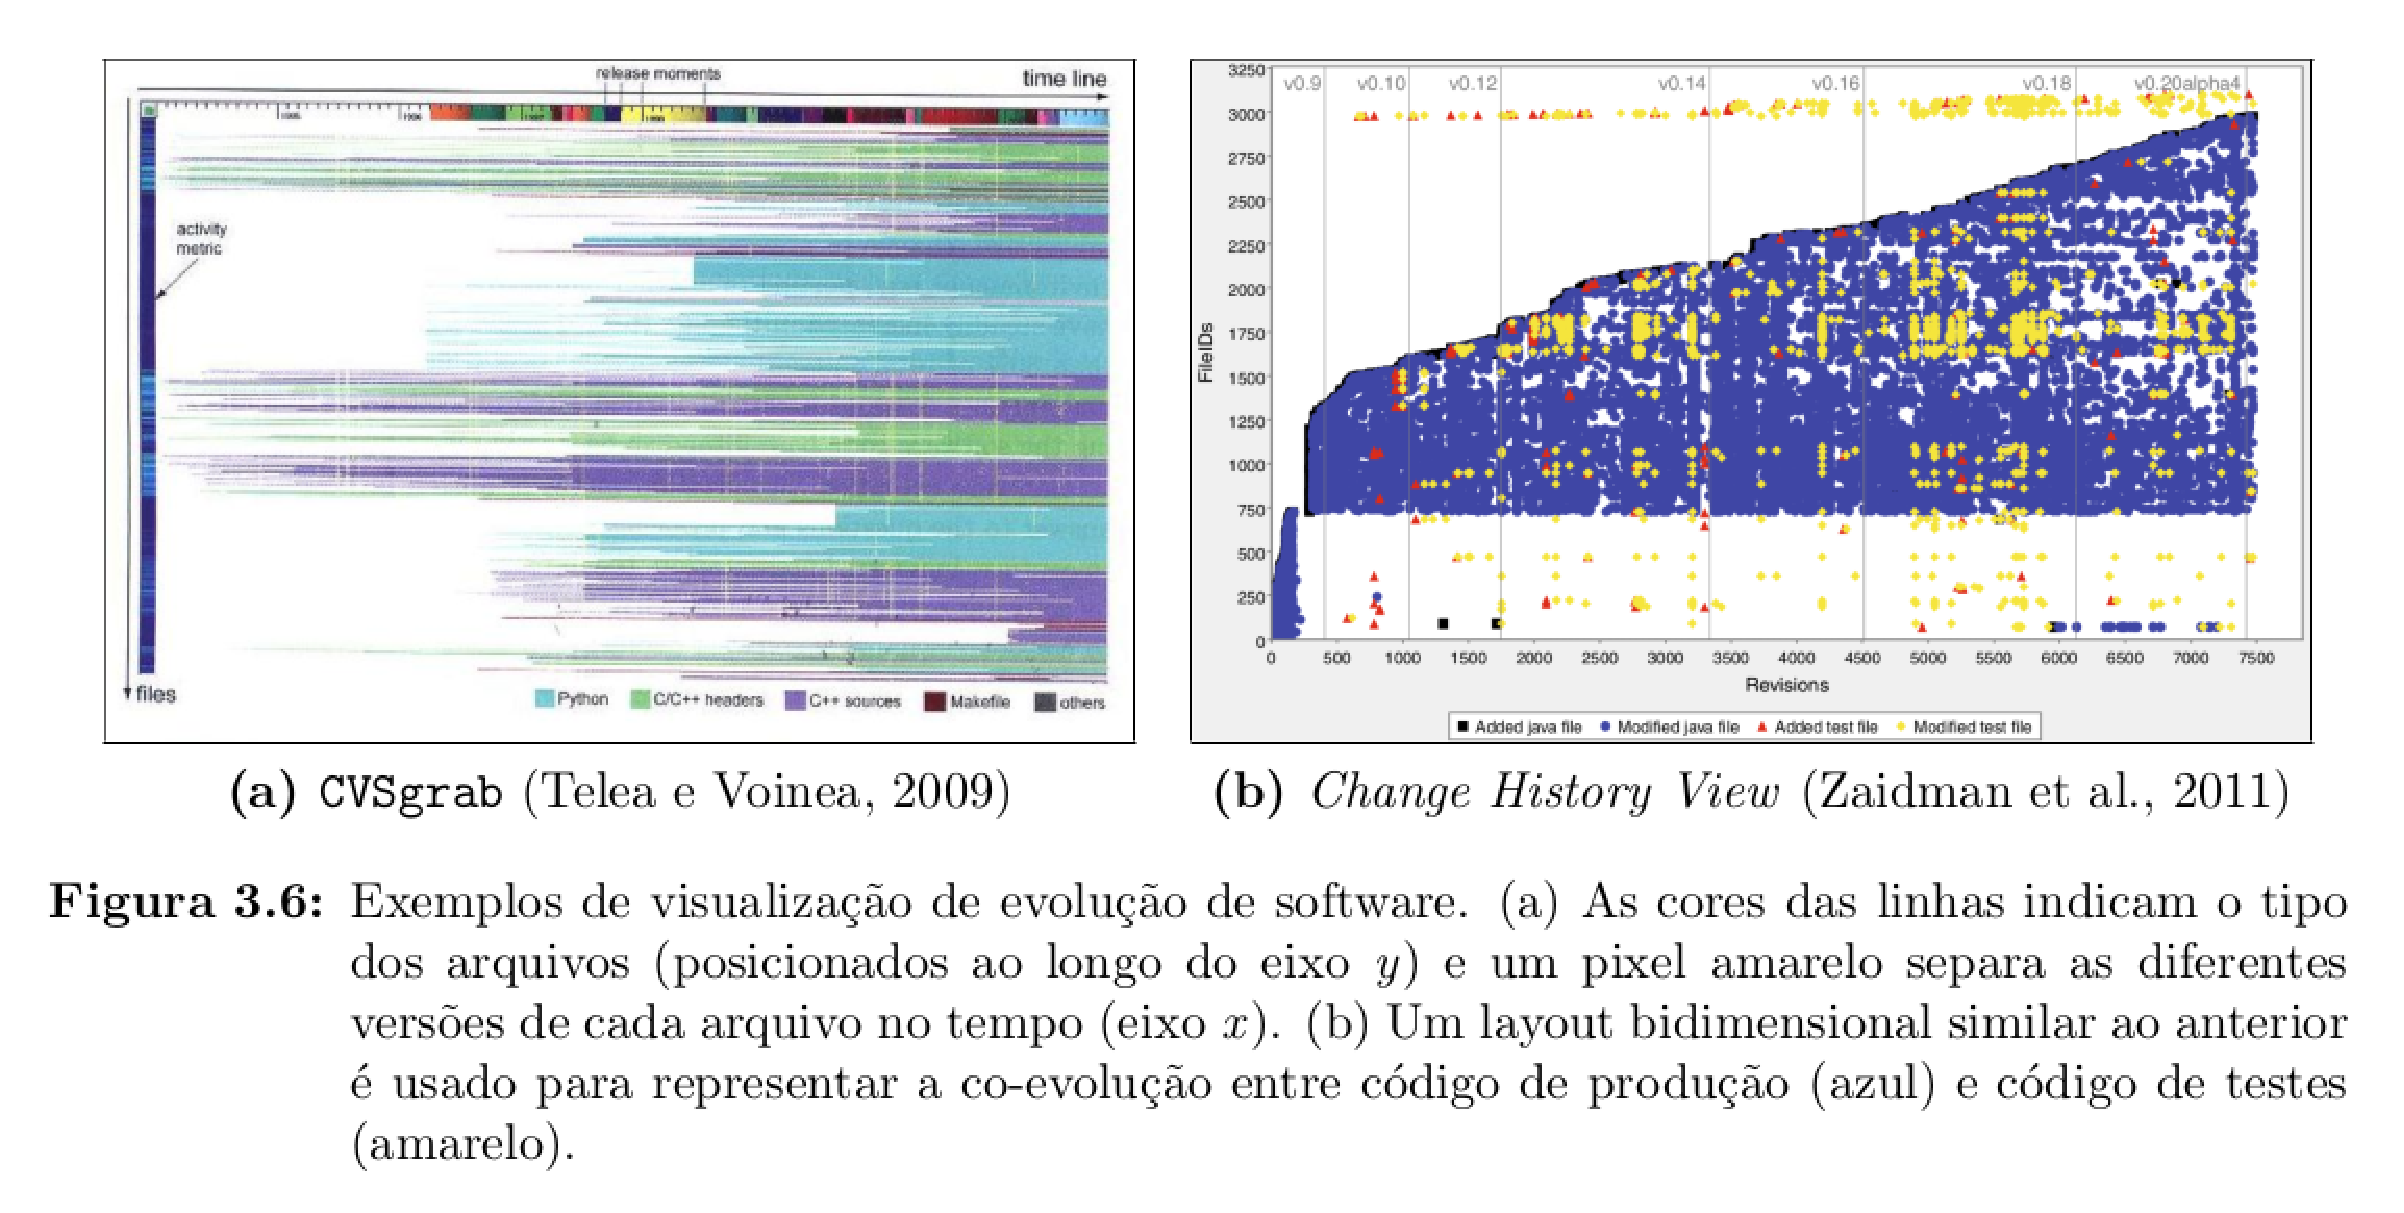
\includegraphics[keepaspectratio=true,scale=0.26]
    {../figuras/exemplo_evolucao.eps}
  \caption{Exemplo Categoria Evolução \cite{messias2012}}
  \label{fig:parallel}
\end{figure}


\end{frame}

%------------------------------------------------
\section{O Mezuro} % Sections can be created in order to organize your presentation into discrete blocks, all sections and subsections are automatically printed in the table of contents as an overview of the talk
%------------------------------------------------

\begin{frame}
\frametitle{O Mezuro}

\center
\textbf{Entendendo Métricas de Código} \\
O Mezuro é uma plataforma web livre para avaliação colaborativa de código fonte. Para iniciar a avaliação, basta fornercer a URL do SCMs (GIT ou SVN). São avaliados códigos escritos em:
\begin{itemize}
\item C, C++, Java - Analizo
\item Ruby - metric\_fu
\item Python - Radon
\end{itemize}

\end{frame}

%------------------------------------------------

\begin{frame}
\frametitle{O Mezuro}

\begin{figure}[!htb]
  \centering
    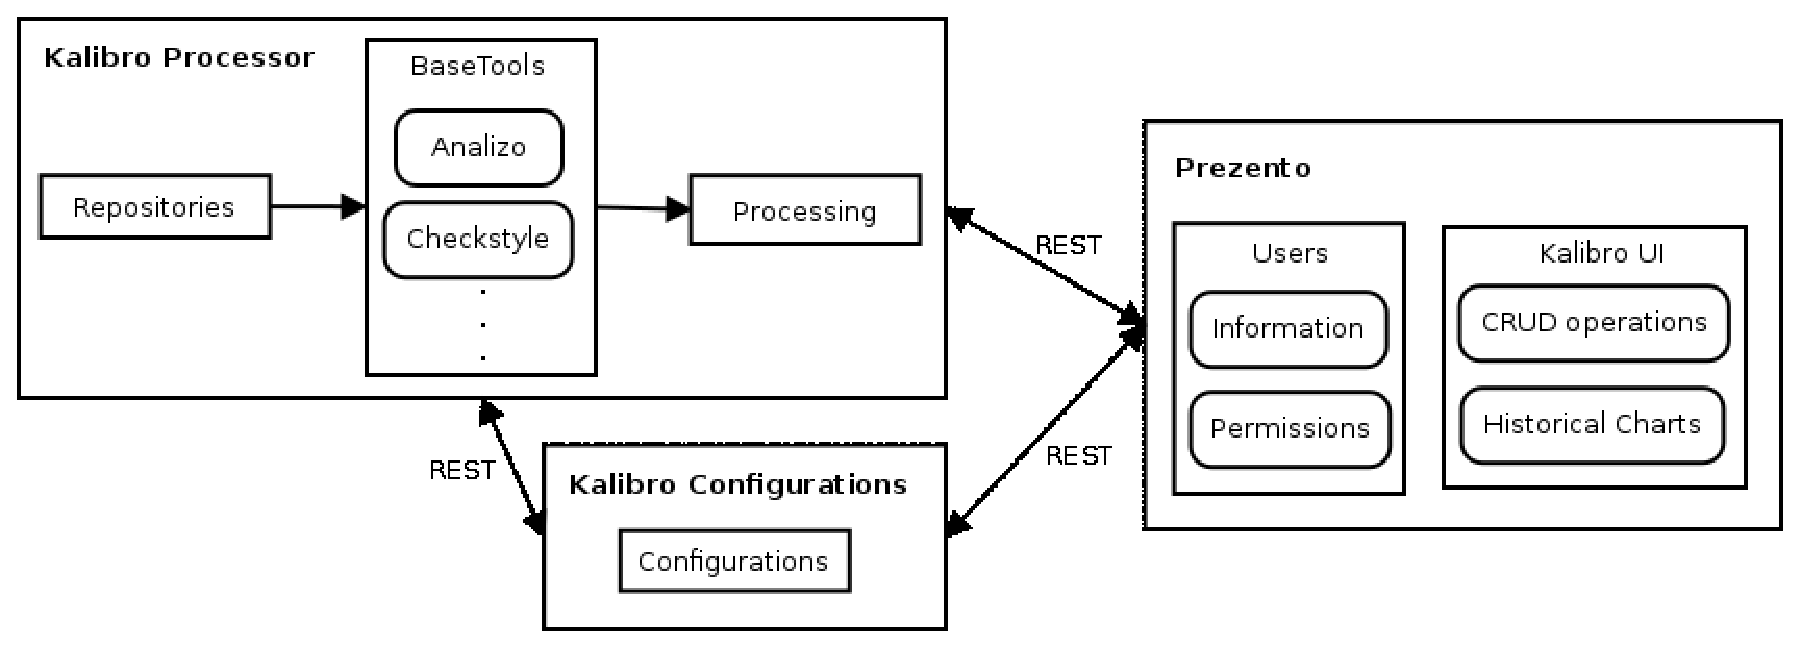
\includegraphics[keepaspectratio=true,scale=0.4]
    {../figuras/mezuroCloudArch.eps}
  \caption{Arquitetura do Mezuro \cite{camarinhaOSS2015}}
  \label{fig:parallel}
\end{figure}

\end{frame}

%------------------------------------------------

\begin{frame}
\frametitle{O Mezuro}

A decisão de utilizar o Mezuro:
\begin{itemize}
\item Aluno já participou da evoulução;
\item Contato com os mantenedores;
\item Plataforma FOSS;
\item Atualização constante.
\end{itemize}

\end{frame}

%------------------------------------------------
\section{Proposta de Evolução da Visualização} % Sections can be created in order to organize your presentation into discrete blocks, all sections and subsections are automatically printed in the table of contents as an overview of the talk
%------------------------------------------------

\begin{frame}
\frametitle{Proposta de Evolução da Visualização}
\begin{itemize}
\item Unir métricas com certo nível similaridade e importância
\item Exibição utilizando as técnicas estudadas;
\end{itemize}
\end{frame}

%------------------------------------------------

\begin{frame}
\frametitle{Proposta de Evolução da Visualização}
\begin{figure}[!htb]
  \centering
    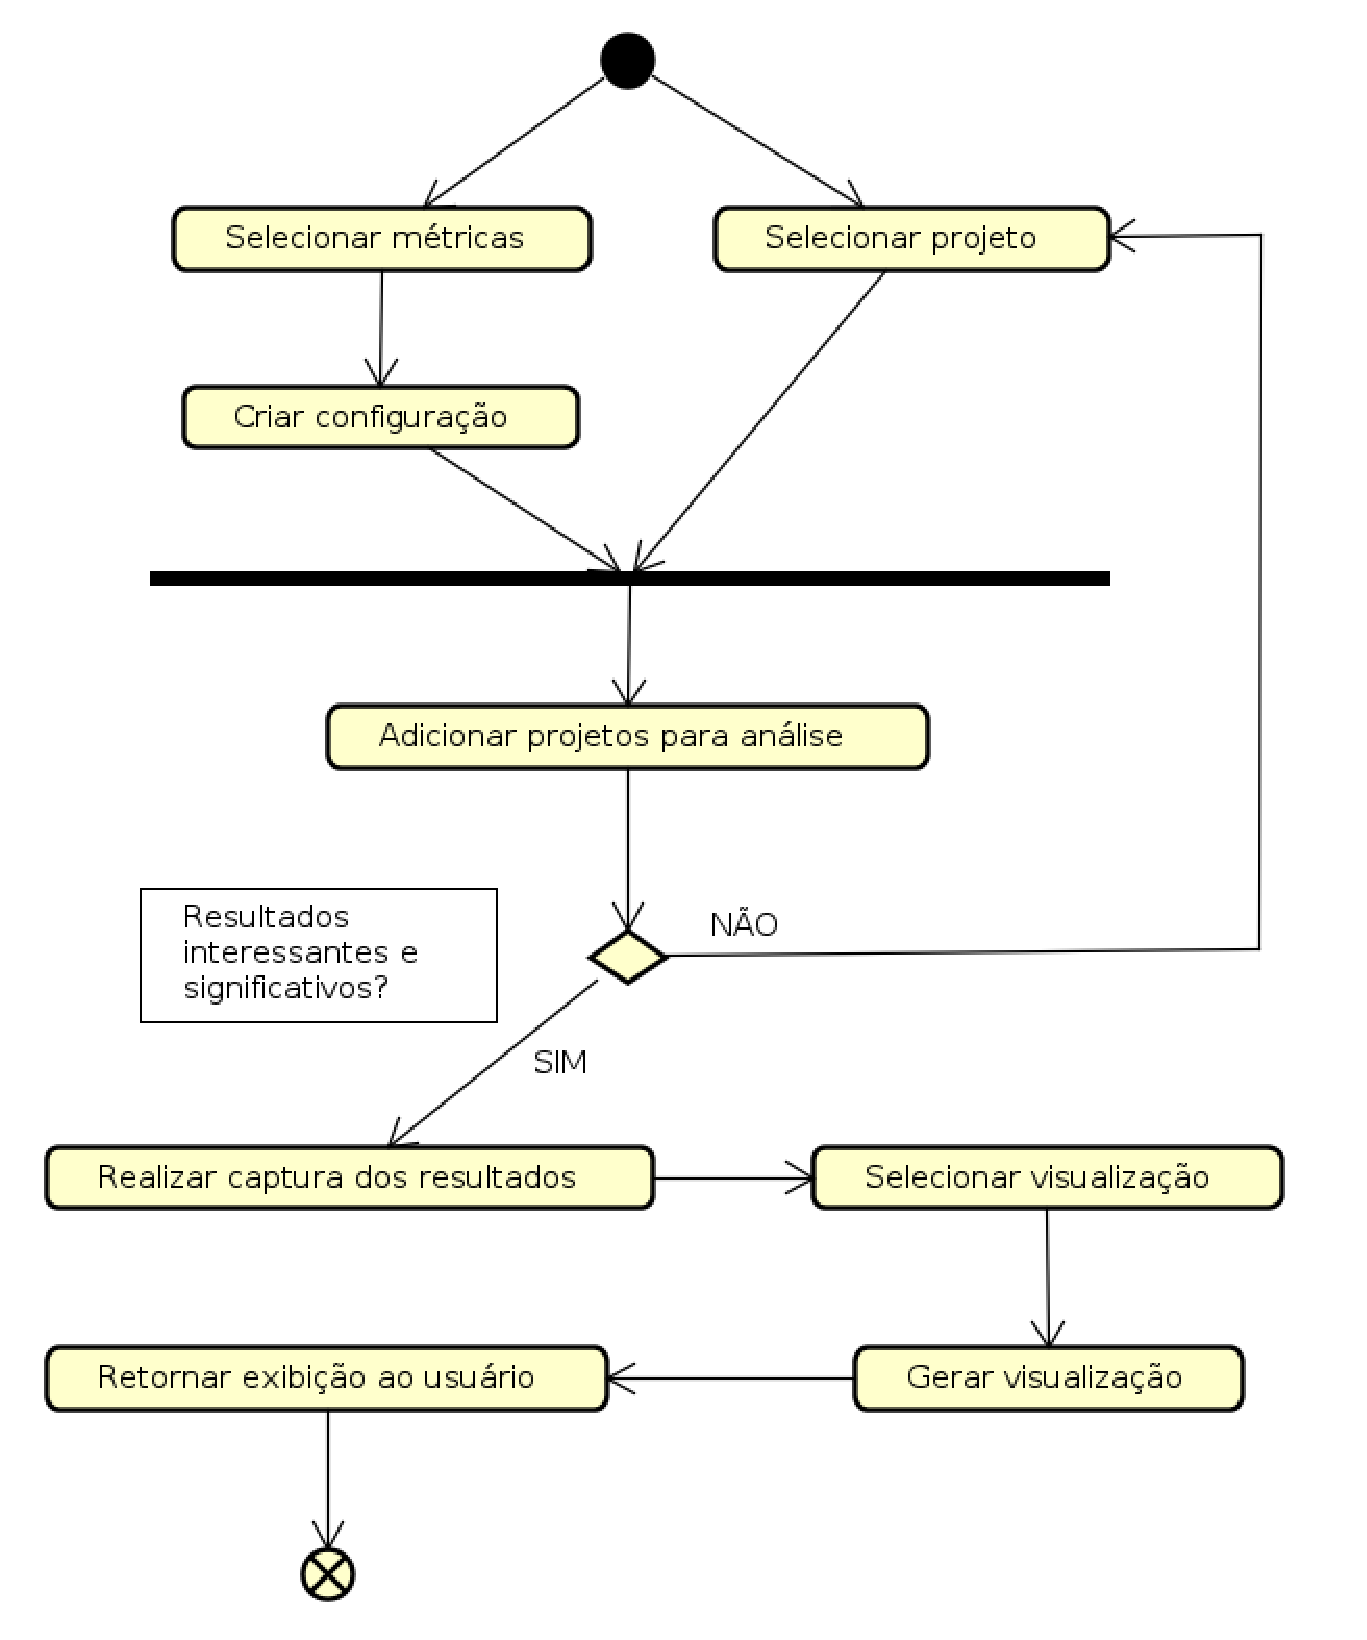
\includegraphics[keepaspectratio=true,scale=0.25]
    {../figuras/metodotologia_atividades.eps}
  \caption{Encadeamento das etapas da atividade de contribuição tecnológica}
  \label{fig:parallel}
\end{figure}
\end{frame}

%------------------------------------------------

\begin{frame}
\frametitle{Proposta de Evolução da Visualização}
\begin{figure}[!htb]
  \centering
    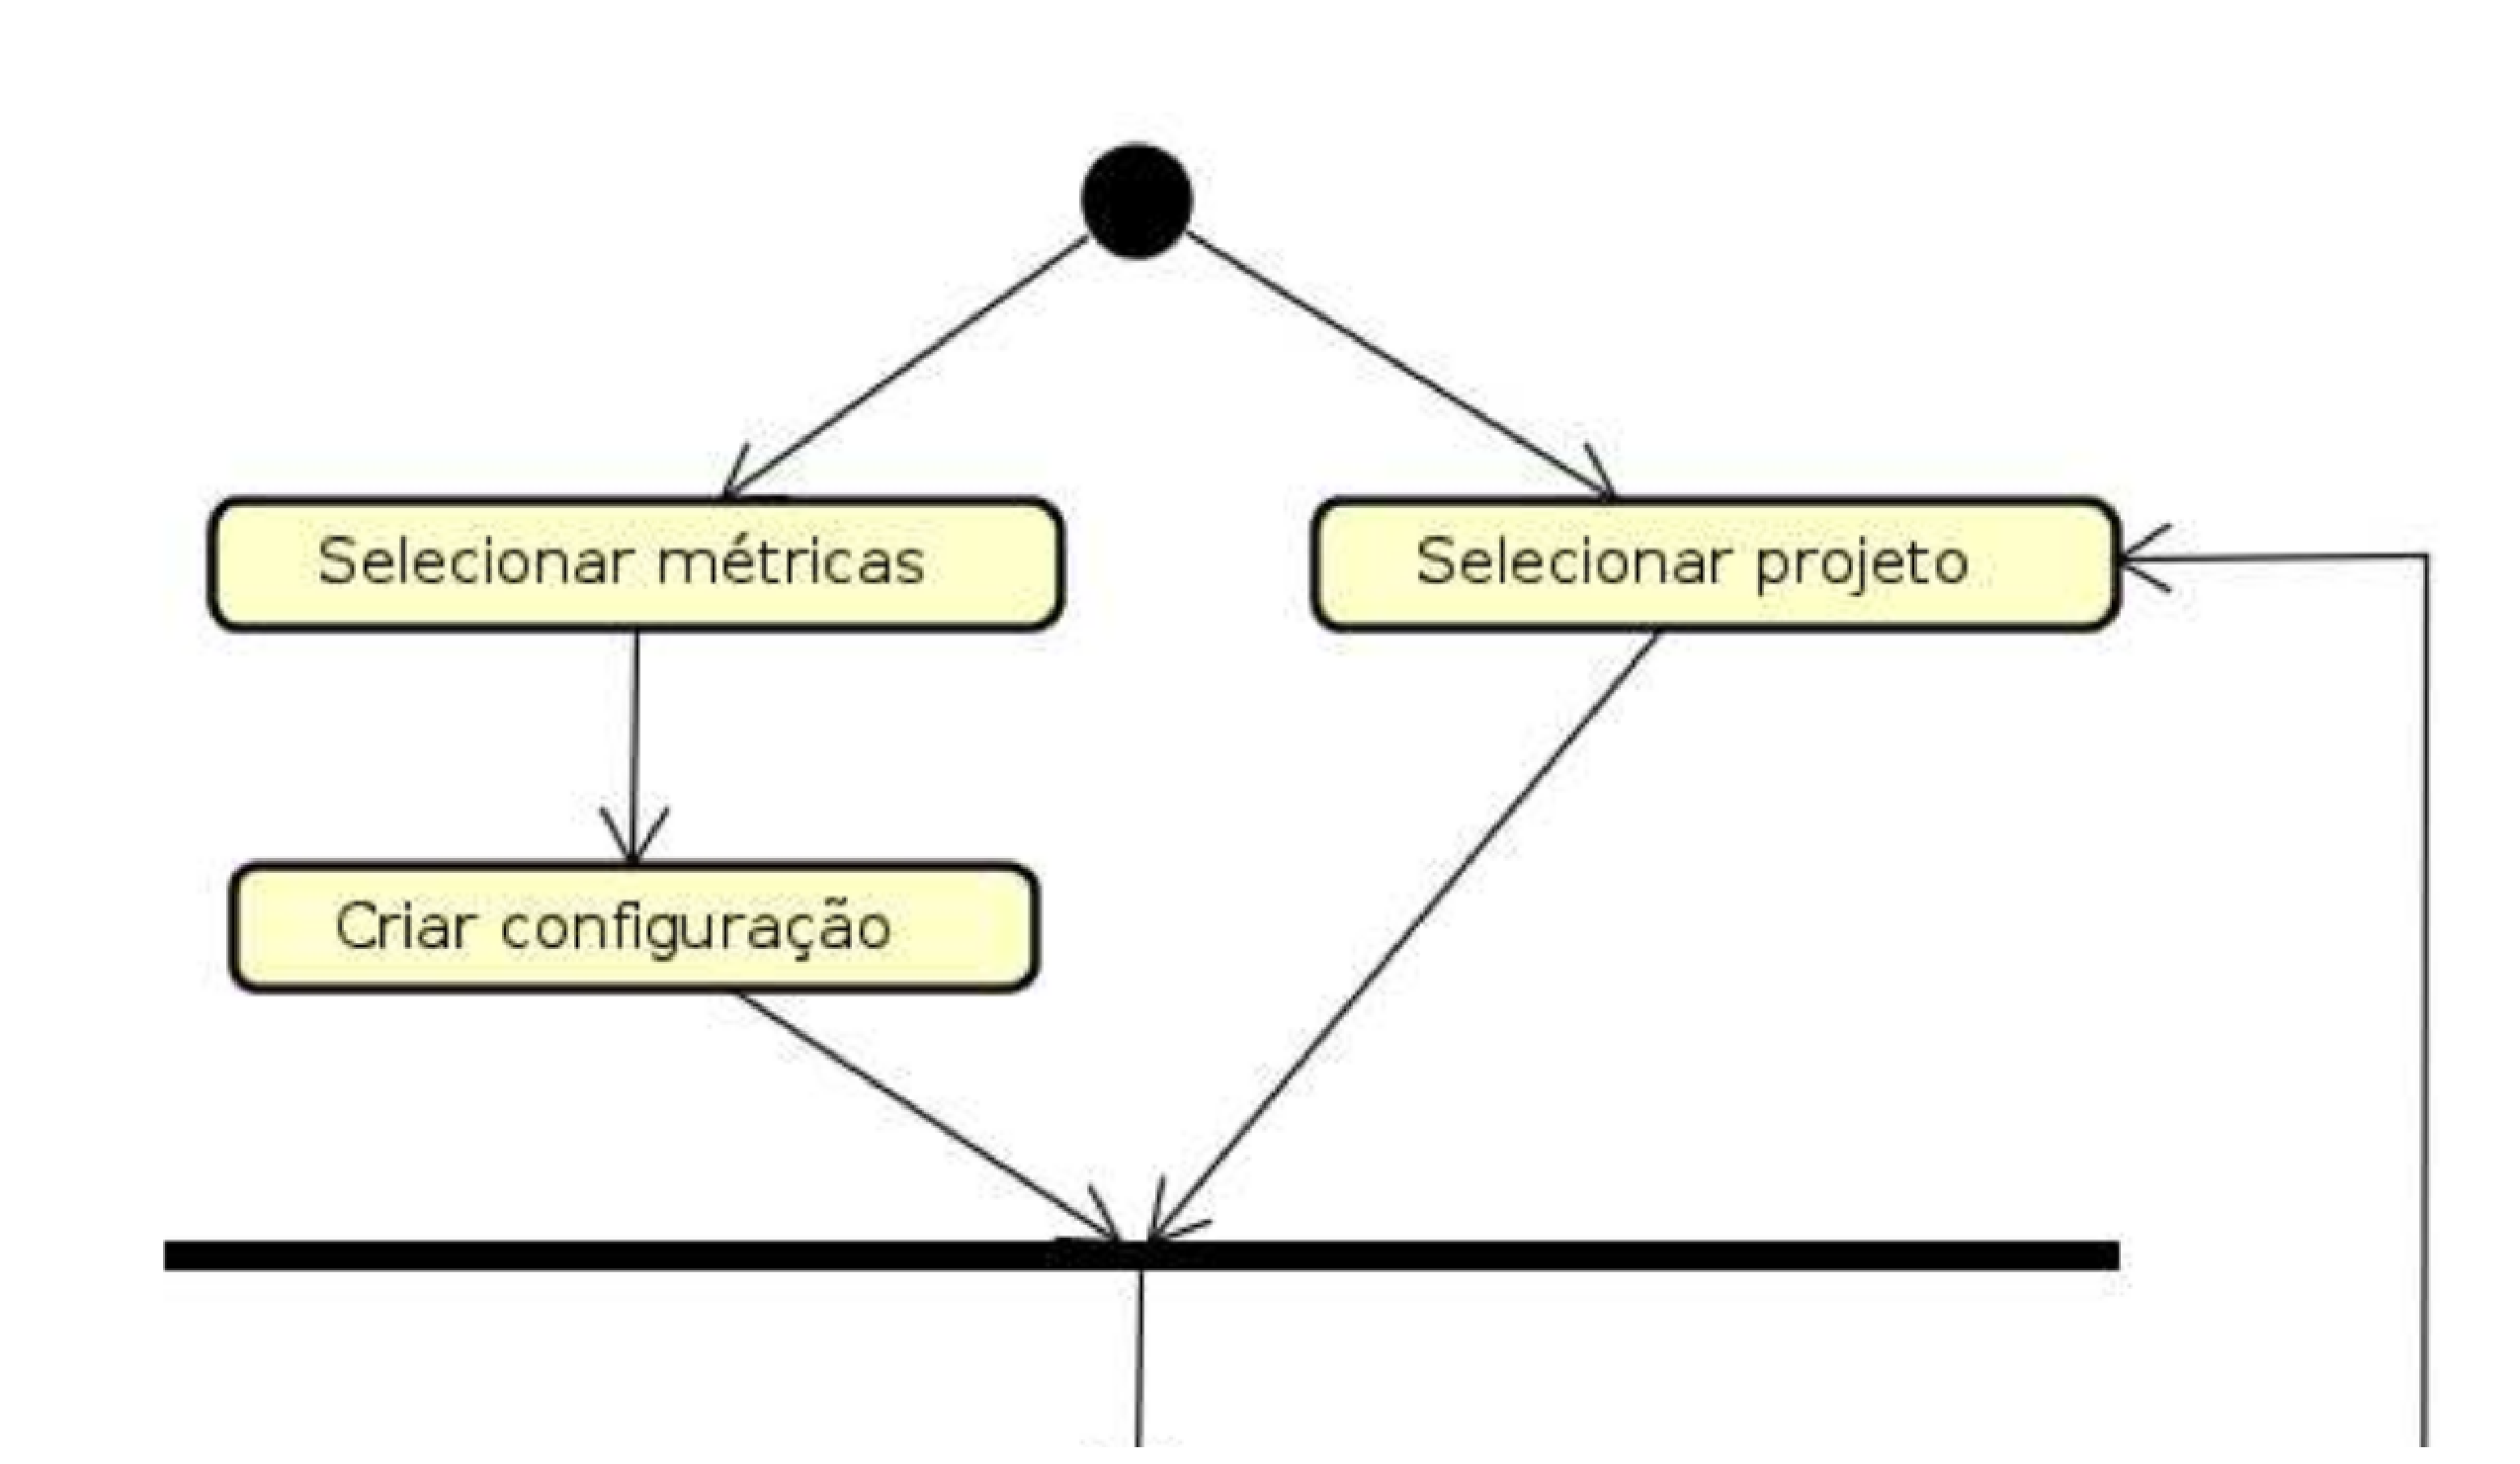
\includegraphics[keepaspectratio=true,scale=0.29]
    {../figuras/encadeamento_1.eps}
  \caption{Encadeamento das etapas da atividade de contribuição tecnológica}
  \label{fig:parallel}
\end{figure}
\end{frame}

%------------------------------------------------

\begin{frame}
\frametitle{Proposta de Evolução da Visualização}
\begin{figure}[!htb]
  \centering
    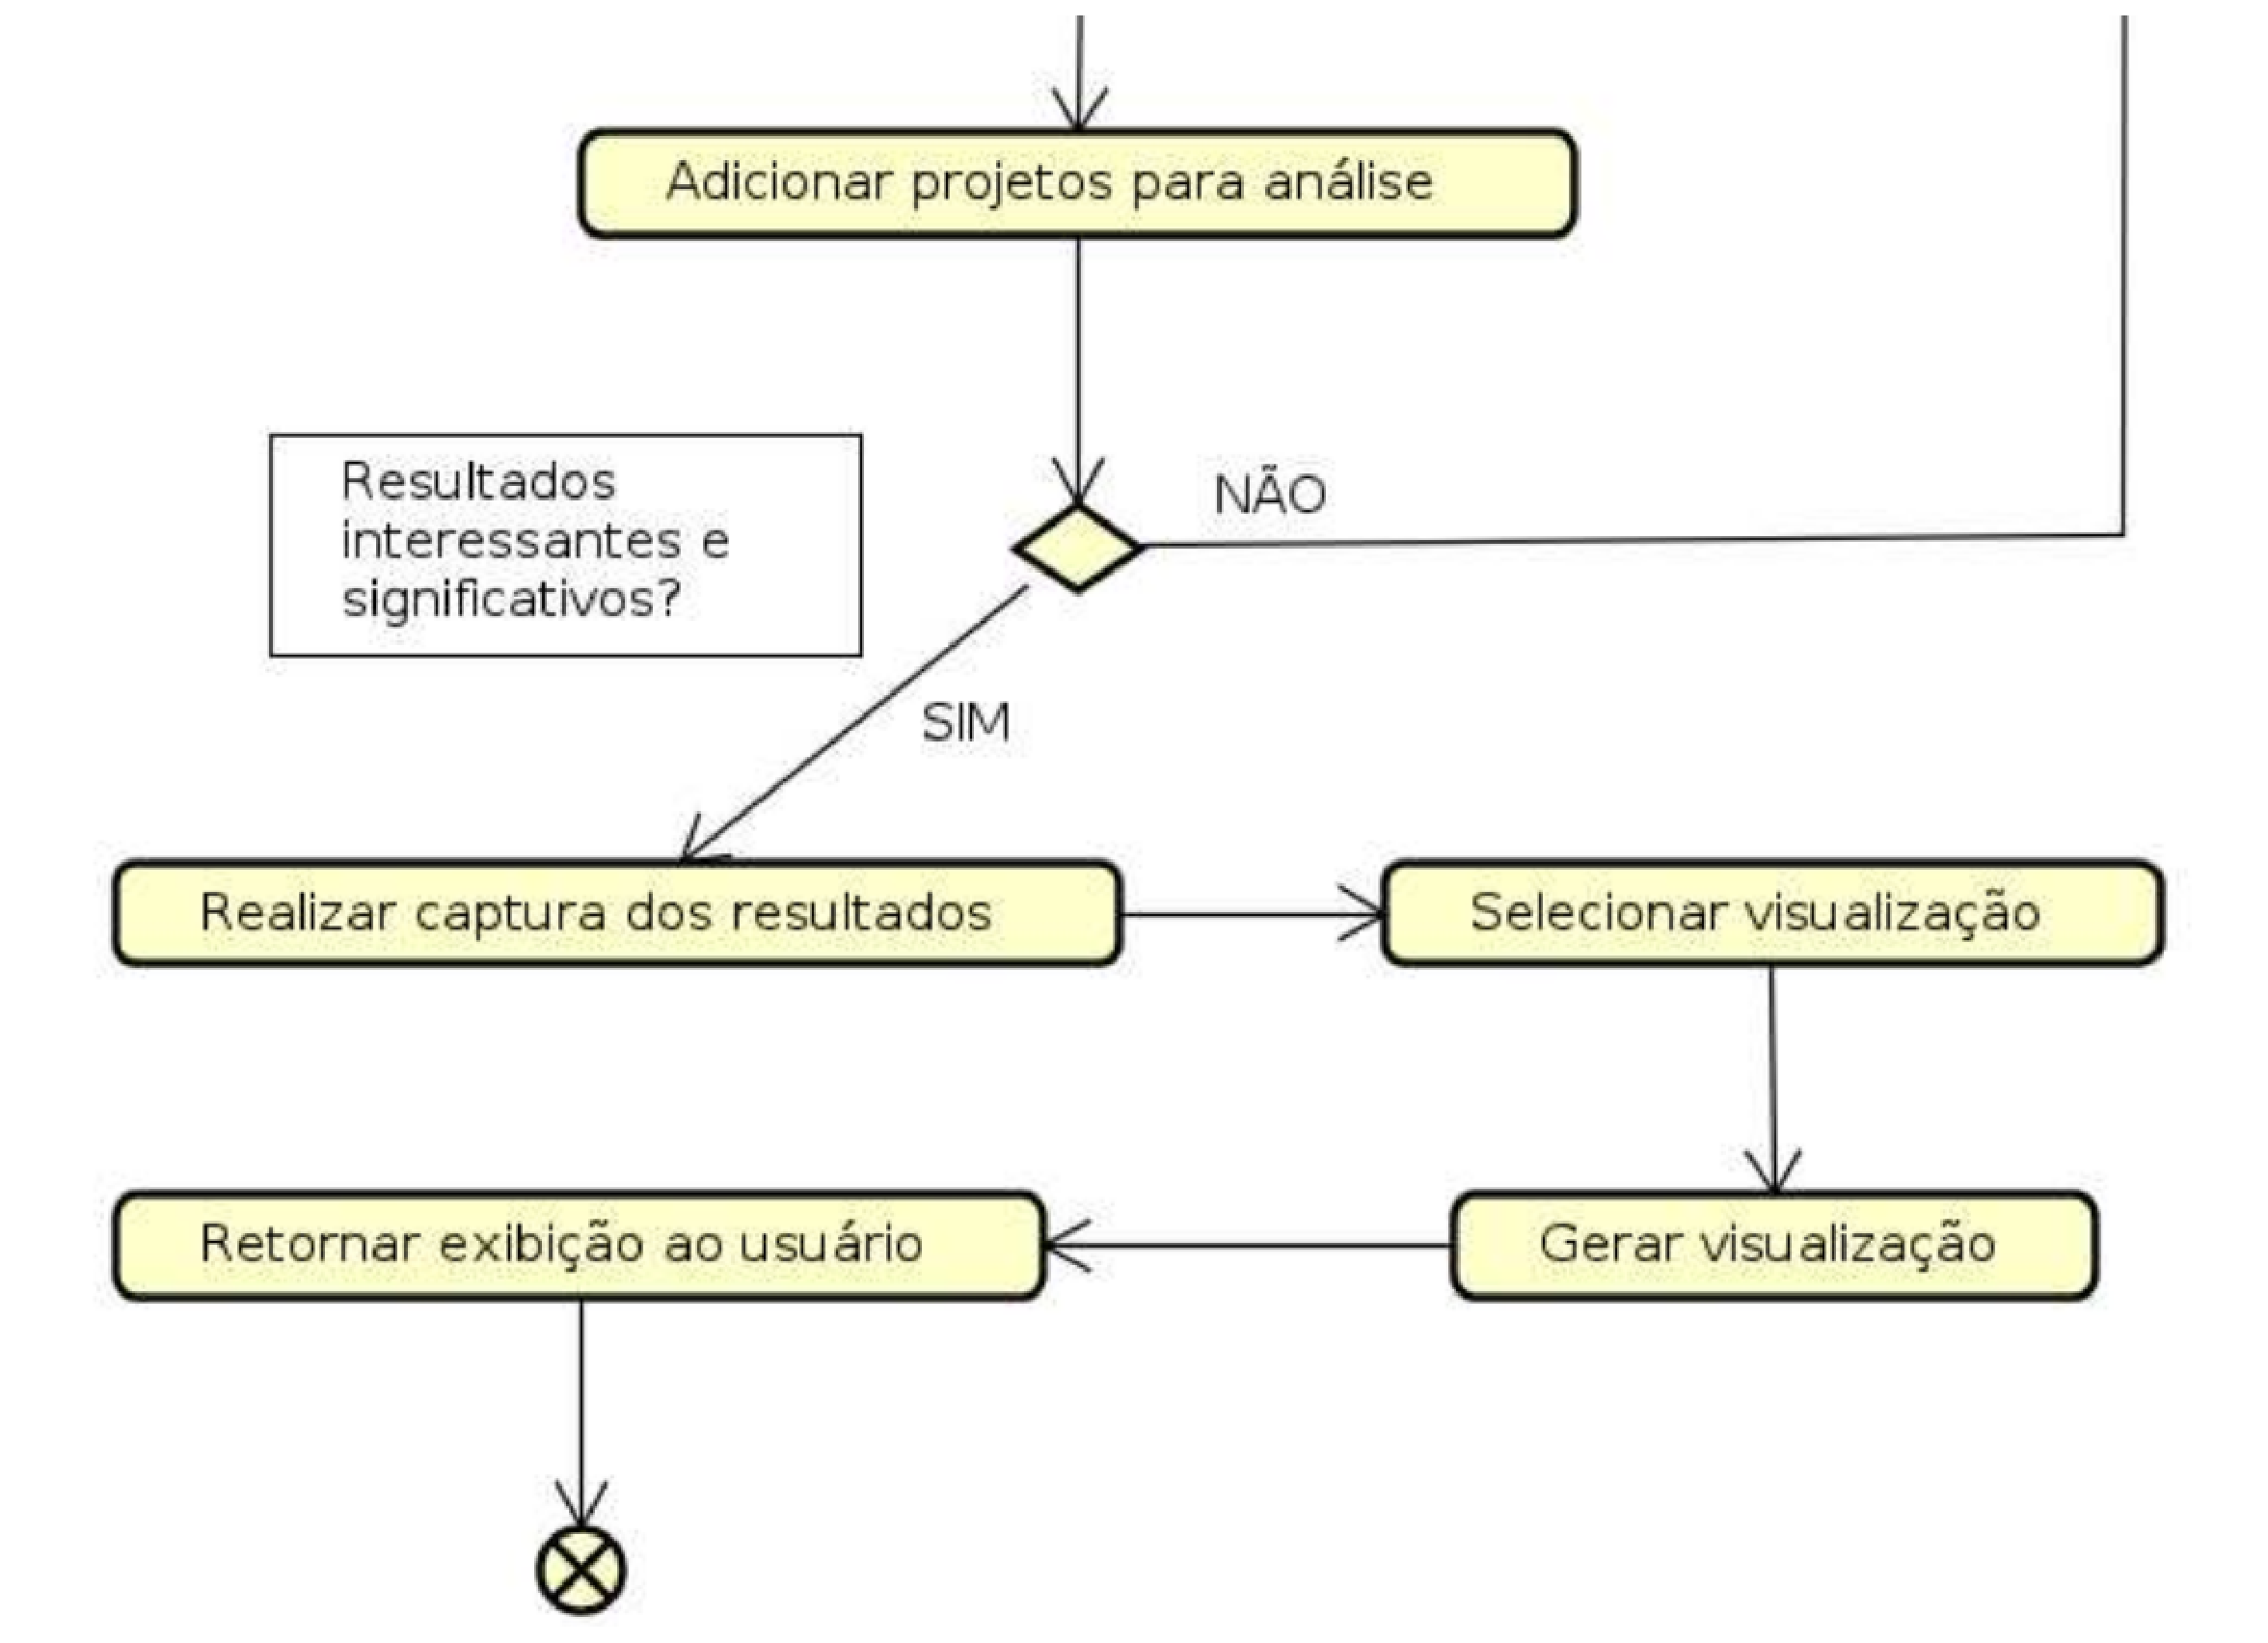
\includegraphics[keepaspectratio=true,scale=0.27]
    {../figuras/encadeamento_2.eps}
  \caption{Encadeamento das etapas da atividade de contribuição tecnológica}
  \label{fig:parallel}
\end{figure}
\end{frame}

%------------------------------------------------
\section{Resultados Preliminares} % Sections can be created in order to organize your presentation into discrete blocks, all sections and subsections are automatically printed in the table of contents as an overview of the talk
%------------------------------------------------

\begin{frame}
\frametitle{Resultados Preliminares}
\textbf{Mezuro - Prezento}
\begin{itemize}
\item GUI
\item Ruby: 2.2.3
\item Rails: 4.2.4
\item Principal Camada para este trabalho
\end{itemize}
\end{frame}

%------------------------------------------------

\begin{frame}
\frametitle{Resultados Preliminares}
\textbf{Possibilidades de disposição dos resultados da VS}
\begin{itemize}
\item Na mesma página
\item Redirecionamento para uma página exclusiva
\end{itemize}
\end{frame}

%------------------------------------------------

\begin{frame}
\frametitle{Resultados Preliminares}
\begin{figure}[!htb]
  \centering
    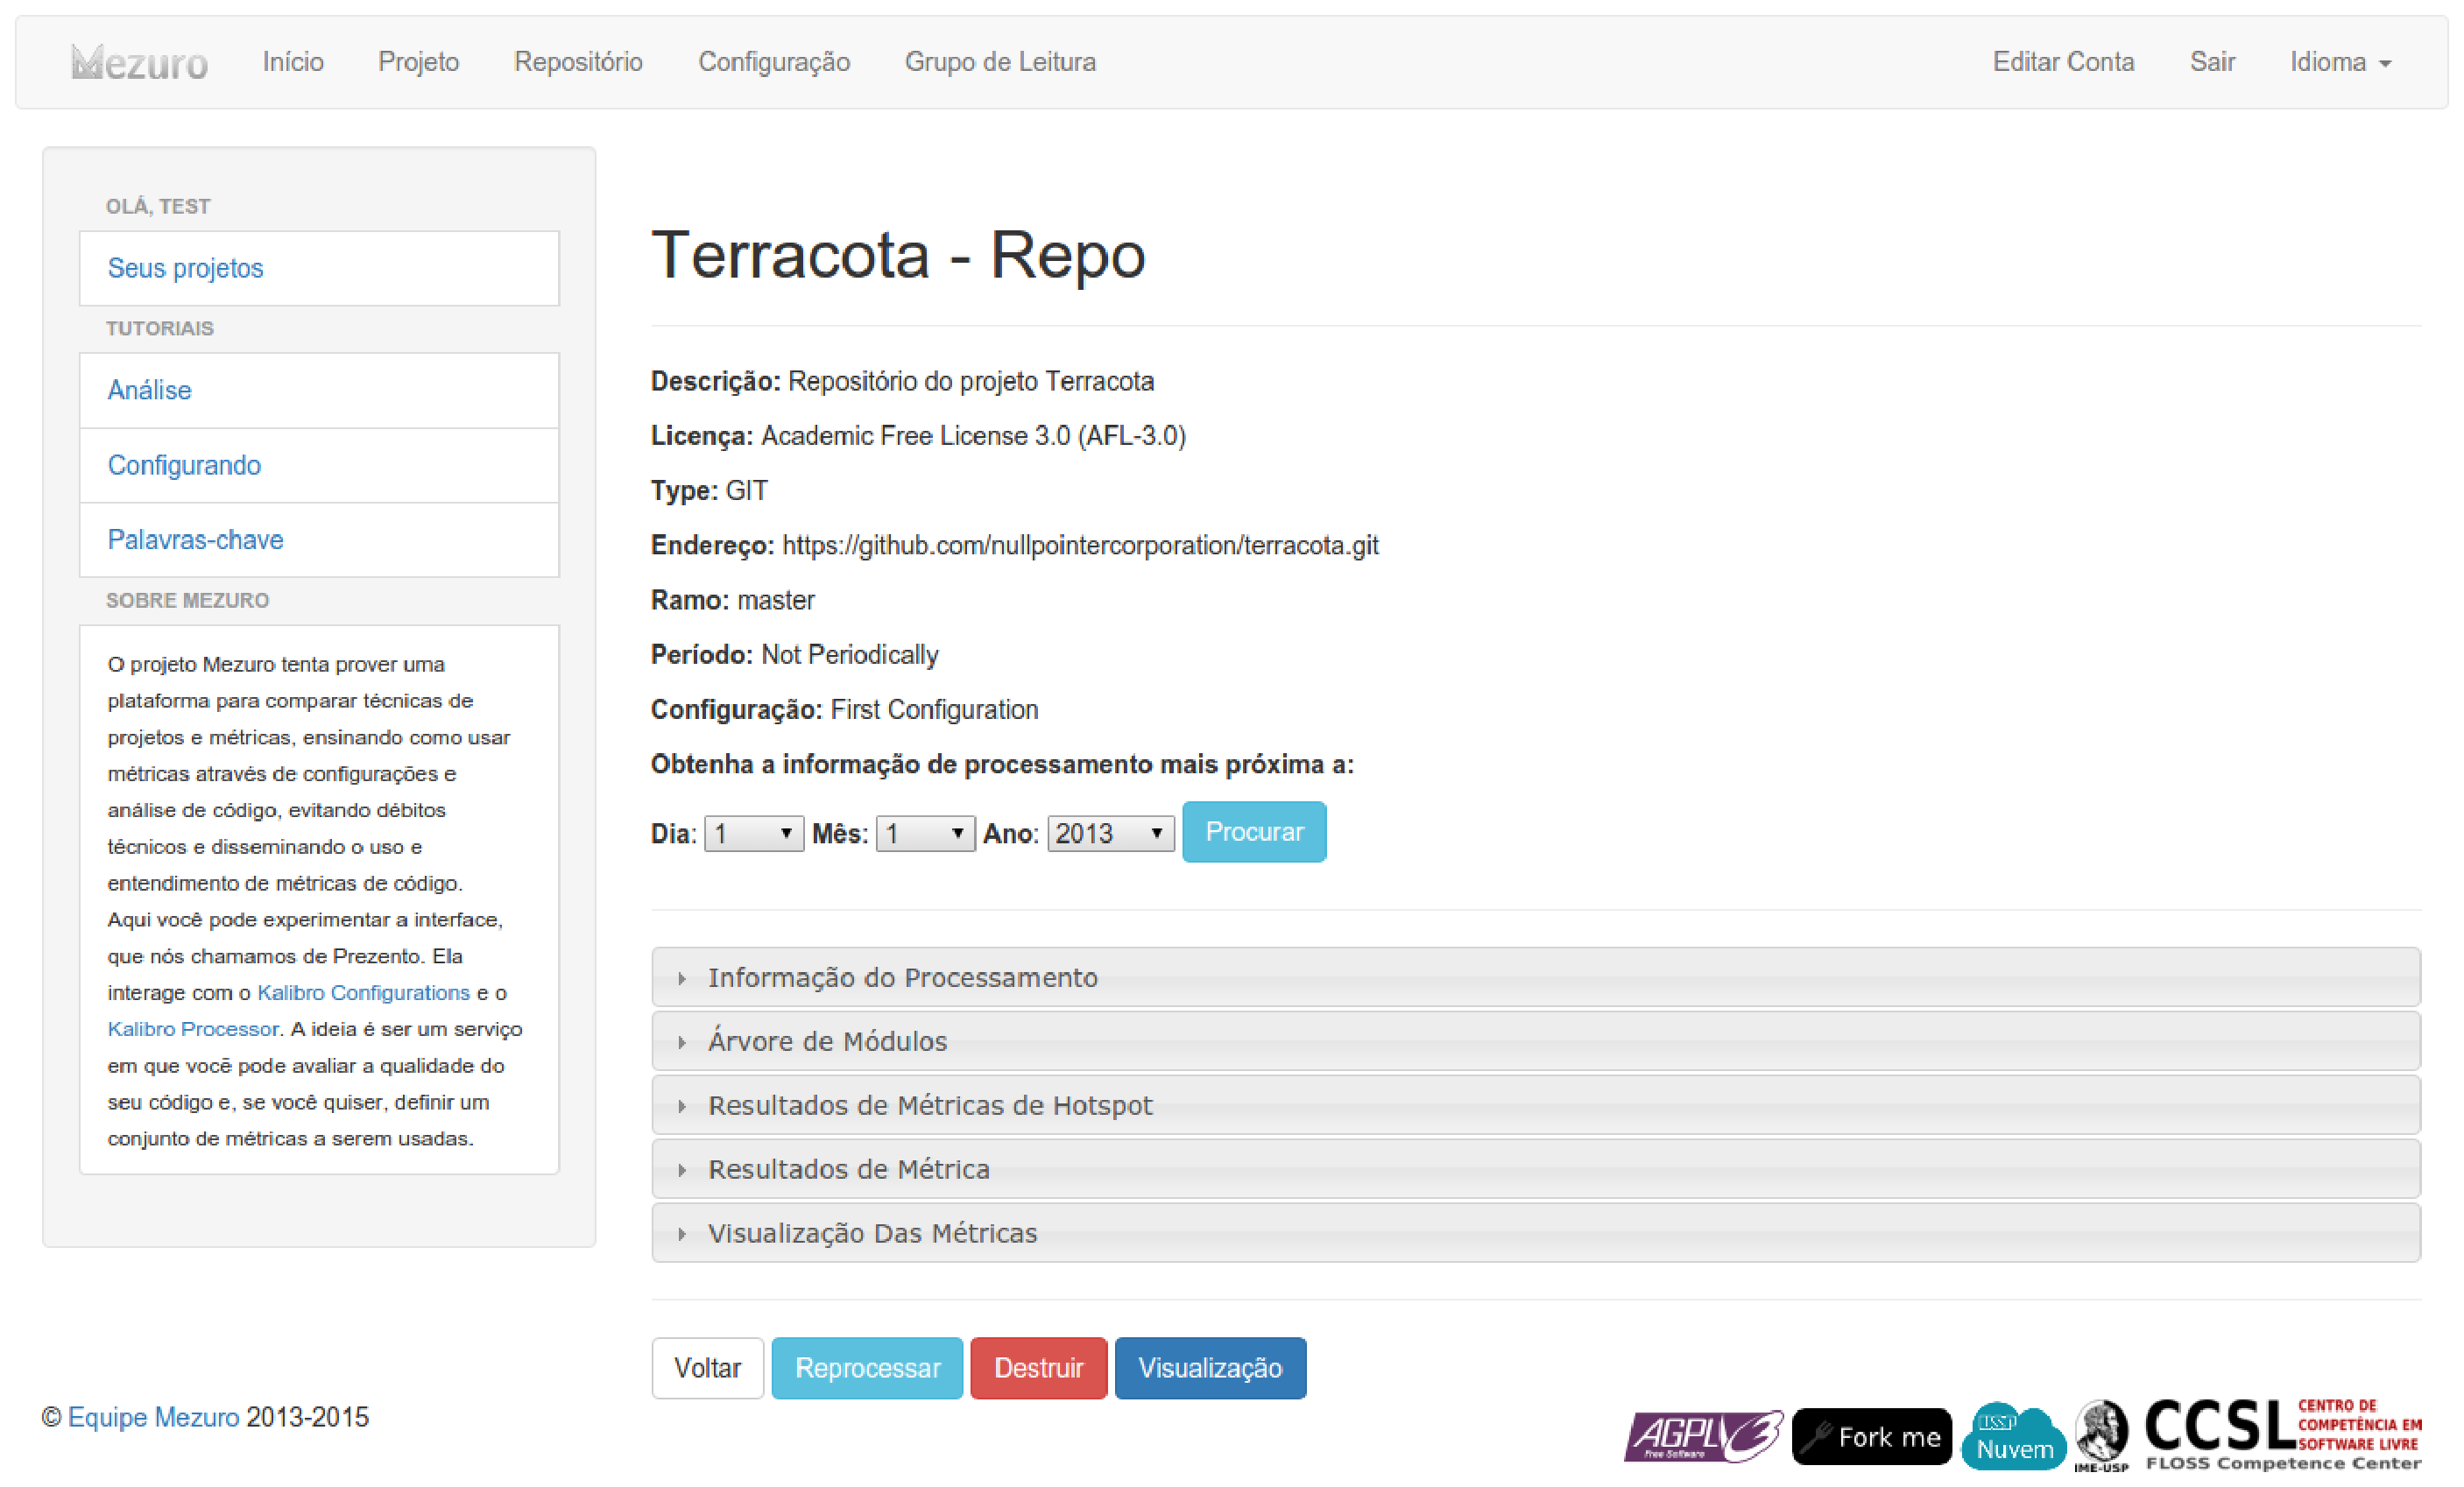
\includegraphics[keepaspectratio=true,scale=0.25]
    {../figuras/exmplo_disposicao_botao_visualizacao_1.eps}
  \caption{Possíveis disposições dos botões de acesso à visualização (recolhido)}
  \label{fig:parallel}
\end{figure}
\end{frame}

%------------------------------------------------

\begin{frame}
\frametitle{Resultados Preliminares}
\begin{figure}[!htb]
  \centering
    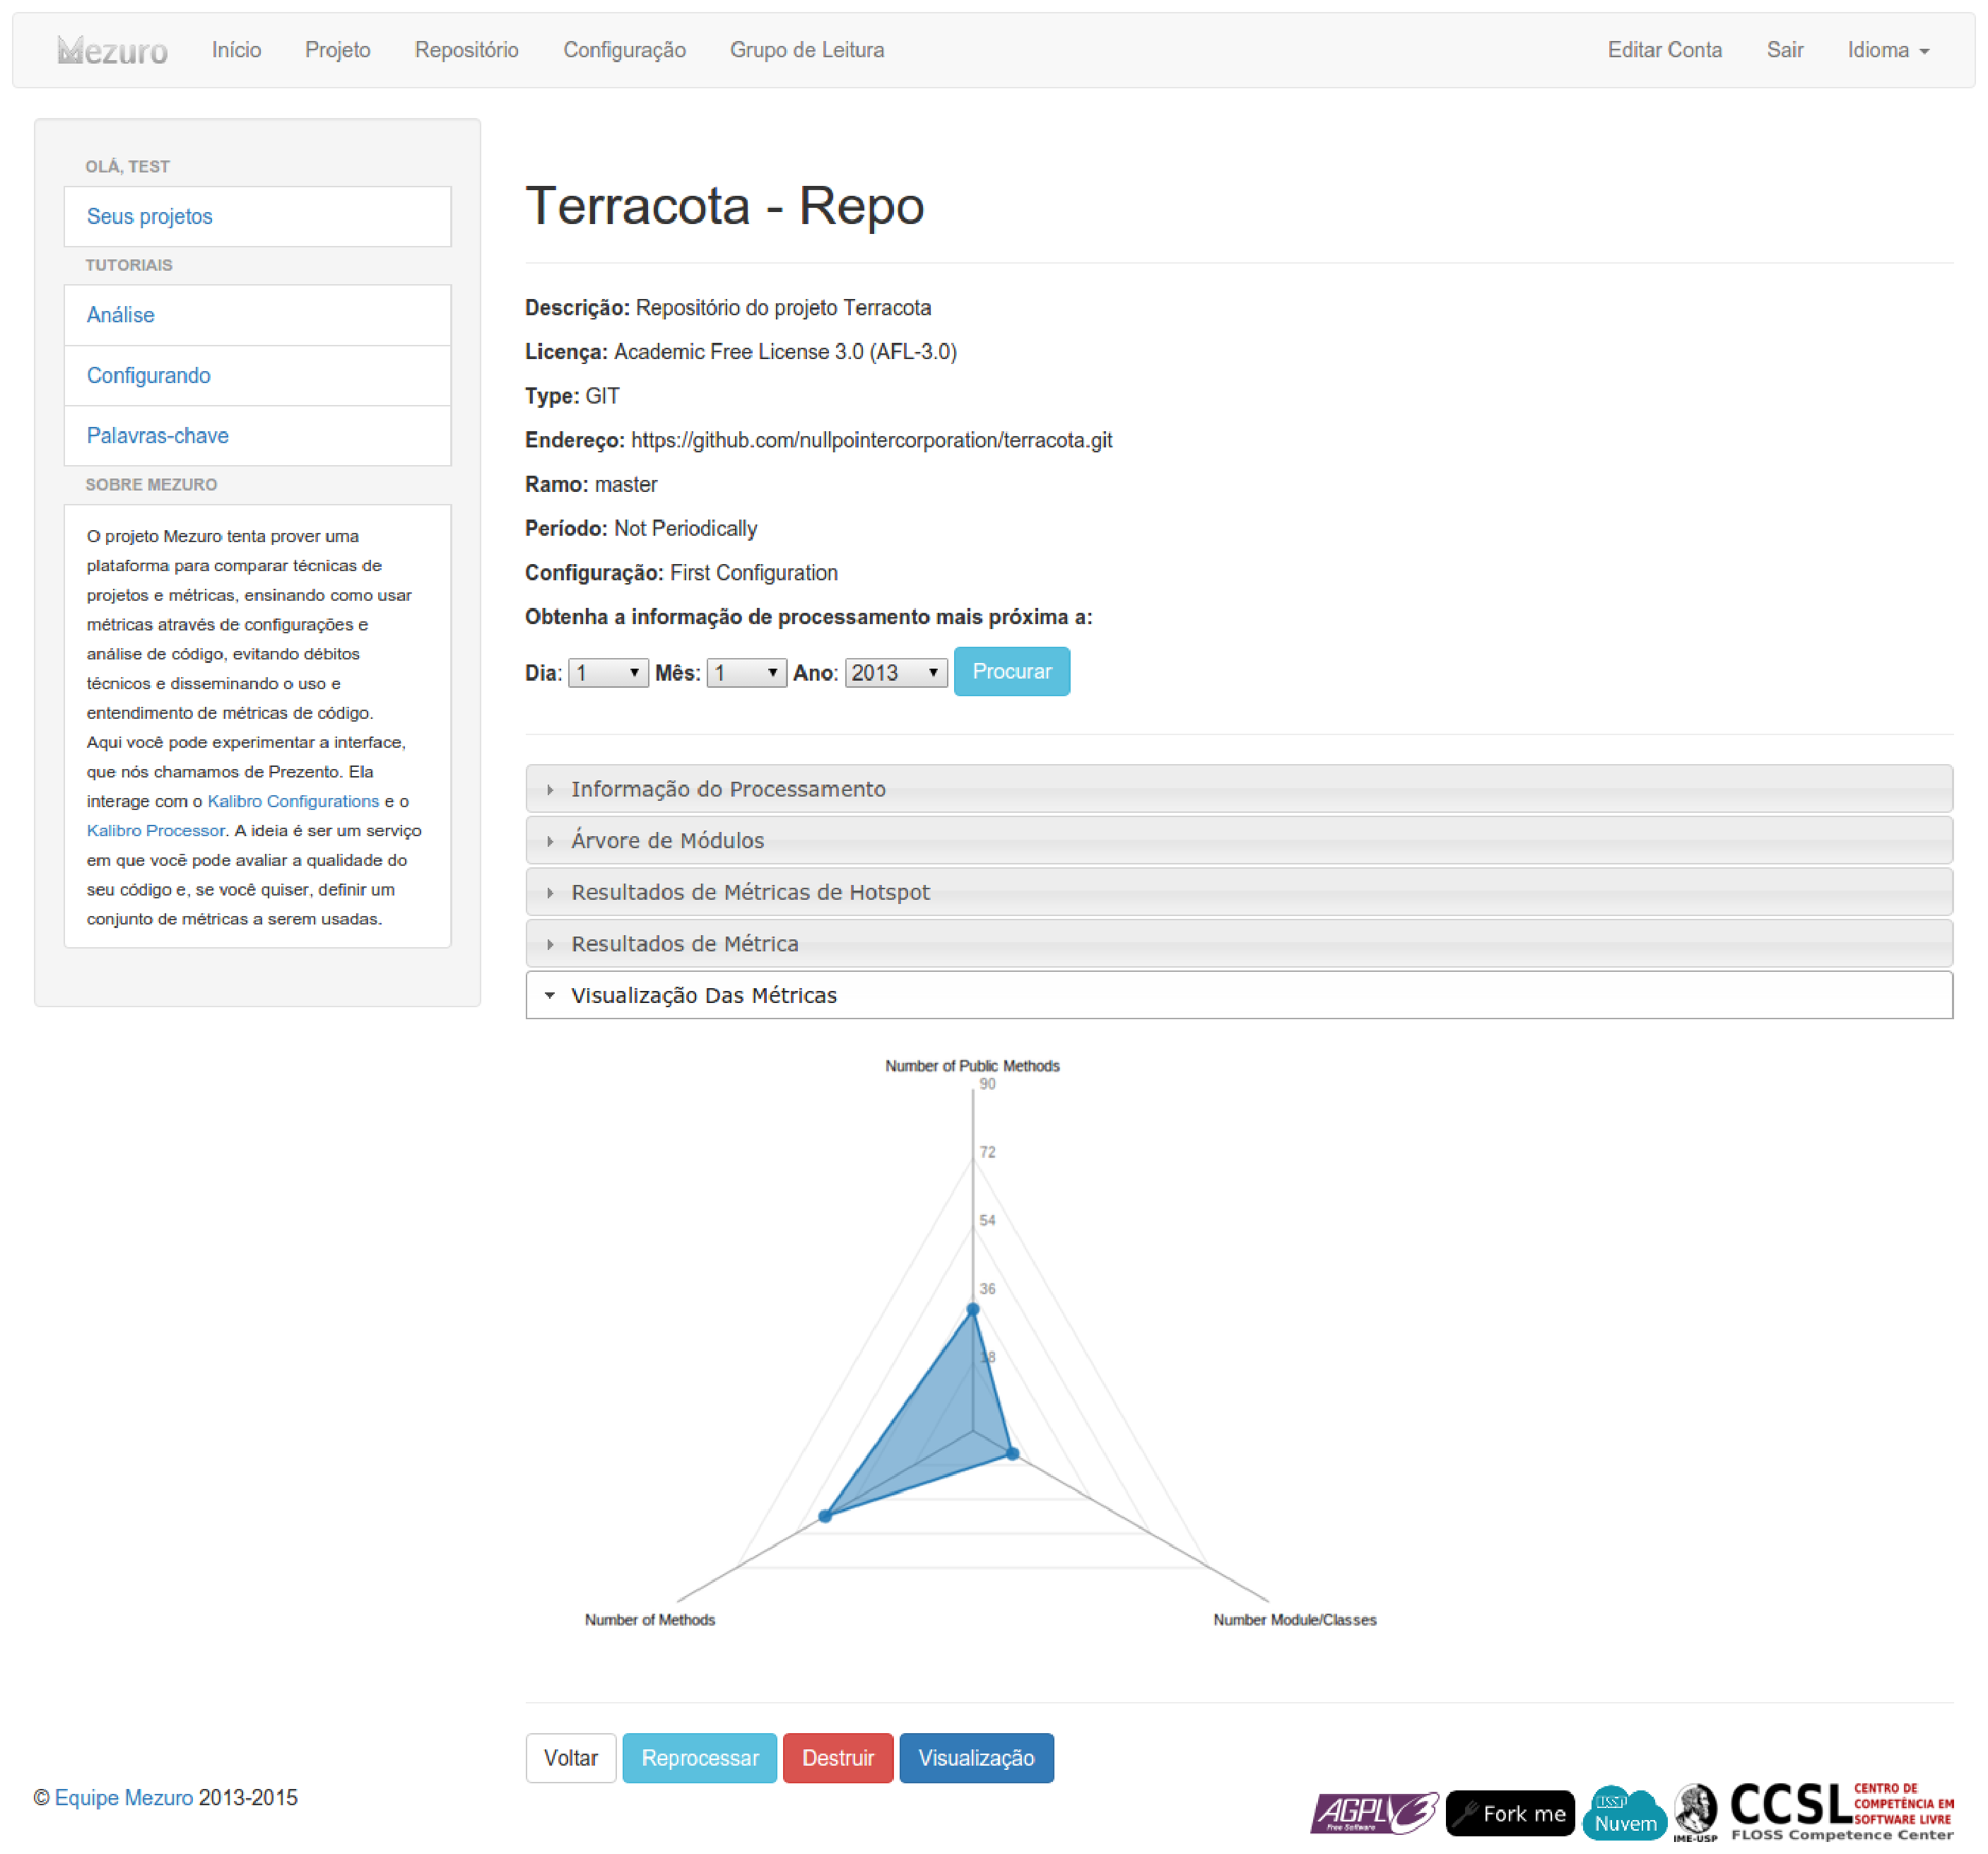
\includegraphics[keepaspectratio=true,scale=0.155]
    {../figuras/exmplo_disposicao_botao_visualizacao_2.eps}
  \caption{Possíveis disposições dos botões de acesso à visualização
  (expandido) (adptado) \cite{filgueiras2014mezuro})}
  \label{fig:parallel}
\end{figure}
\end{frame}

%------------------------------------------------

\begin{frame}
\frametitle{Resultados Preliminares}
\textbf{D3 - Data-Driven Documents}
\begin{figure}[!htb]
  \centering
    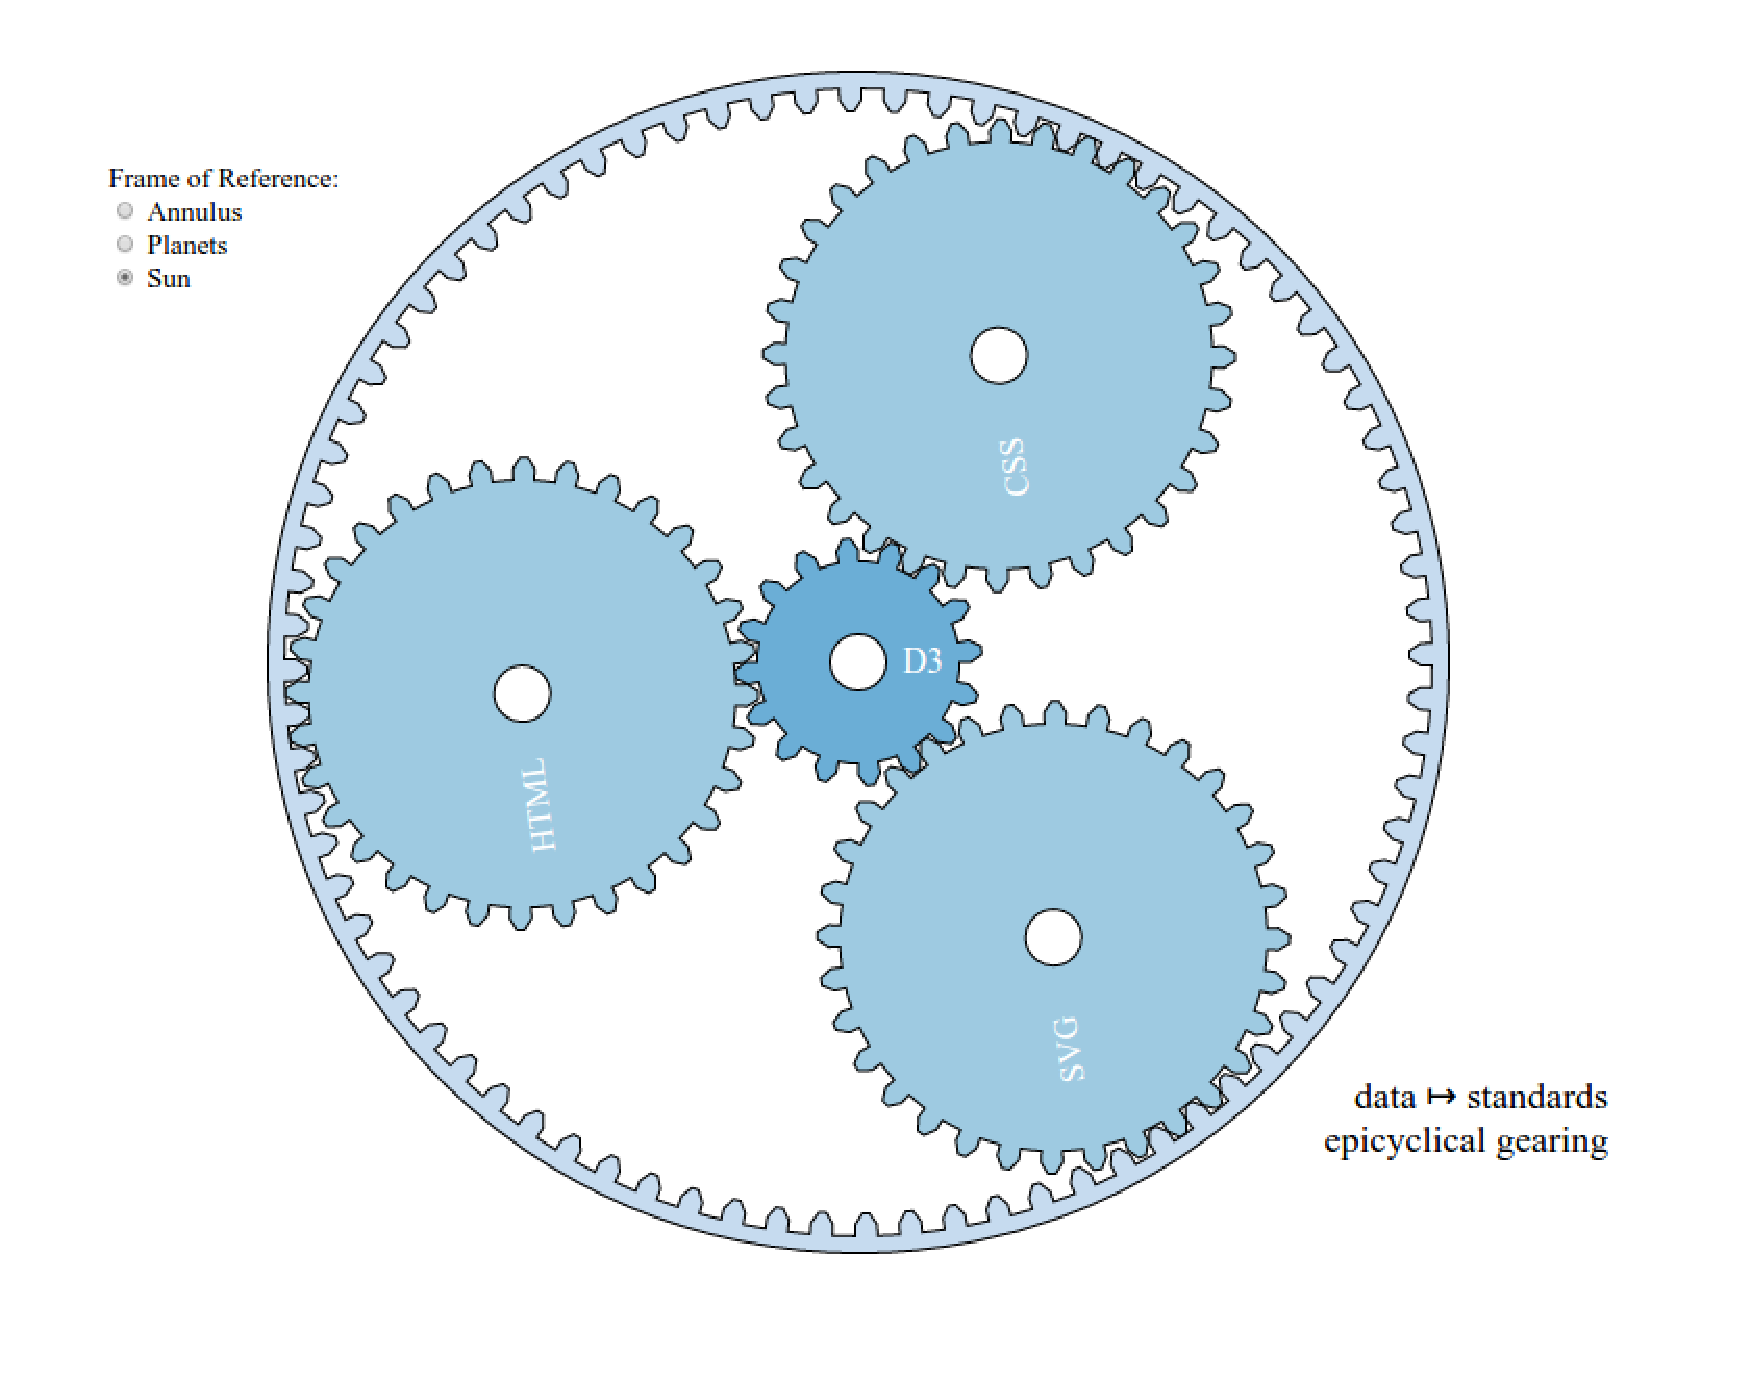
\includegraphics[keepaspectratio=true,scale=0.28]
    {../figuras/d3_gears.eps}
  \caption{Exemplificação do Uso das Tecnologias pela D3.js \cite{michaeld3}}
  \label{fig:parallel}
\end{figure}
\end{frame}

%------------------------------------------------

\begin{frame}
\frametitle{Resultados Preliminares}
\textbf{D3 - Data-Driven Documents}
\begin{itemize}
\item DOM
\item Preocupações: compatibilidade, depuração e desempenho
\item BSD licenses
\item Vasta biblioteca
\end{itemize}
\end{frame}

%------------------------------------------------
\section{Conclusão} % Sections can be created in order to organize your presentation into discrete blocks, all sections and subsections are automatically printed in the table of contents as an overview of the talk
%------------------------------------------------

\begin{frame}
\frametitle{Conclusão}
\textbf{Atividades e Cronograma}

\begin{itemize}
\item Reforço da Revisão Bibliográfica
\item Elaboração
\item Levantamento do Ambiente de Desenvolvimento
\item Desenvolvimento das Visualizações
\item Desenvolvimento e Melhorias
\item Revisão e Escrita
\item Apresentação do TCC2
\end{itemize}

\end{frame}

%------------------------------------------------

\begin{frame}
\frametitle{Conclusão}
\textbf{Atividades e Cronograma}
\begin{figure}[!htb]
  \centering
    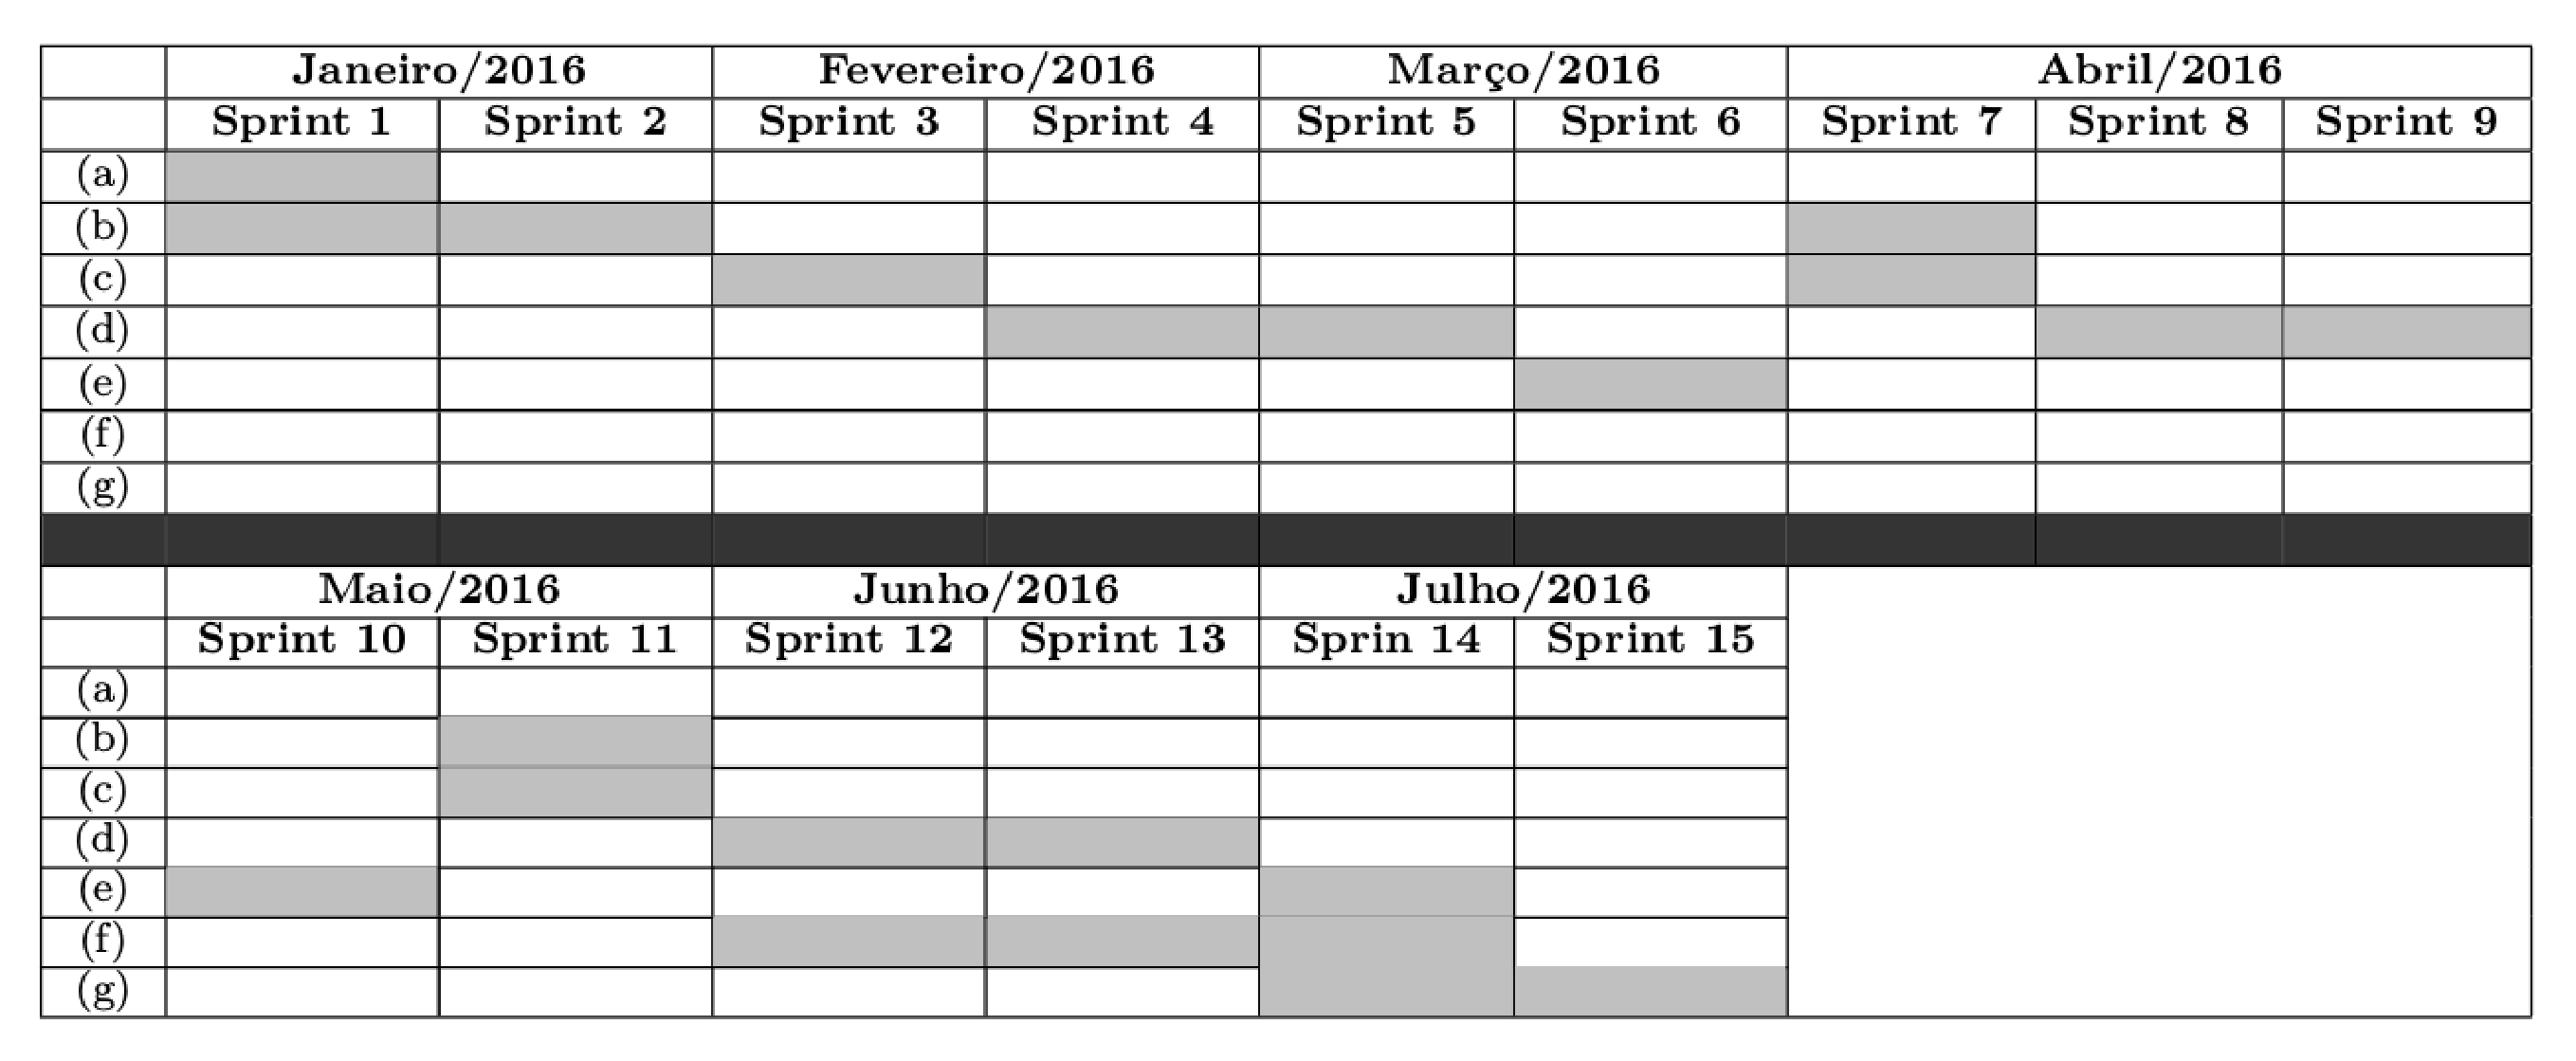
\includegraphics[keepaspectratio=true,scale=0.27]
    {../figuras/print_cronograma.eps}
  \caption{Cronograma}
  \label{fig:parallel}
\end{figure}
\end{frame}

%------------------------------------------------

\begin{frame}
\frametitle{References}
        \bibliographystyle{amsalpha}
        \bibliography{../bibliografia.bib}
\end{frame}

%------------------------------------------------

\begin{frame}
\Huge{\centerline{Obrigado!}}
\end{frame}

%----------------------------------------------------------------------------------------

\end{document}
